% Options for packages loaded elsewhere
\PassOptionsToPackage{unicode}{hyperref}
\PassOptionsToPackage{hyphens}{url}
%
\documentclass[
]{book}
\usepackage{lmodern}
\usepackage{amssymb,amsmath}
\usepackage{ifxetex,ifluatex}
\ifnum 0\ifxetex 1\fi\ifluatex 1\fi=0 % if pdftex
  \usepackage[T1]{fontenc}
  \usepackage[utf8]{inputenc}
  \usepackage{textcomp} % provide euro and other symbols
\else % if luatex or xetex
  \usepackage{unicode-math}
  \defaultfontfeatures{Scale=MatchLowercase}
  \defaultfontfeatures[\rmfamily]{Ligatures=TeX,Scale=1}
\fi
% Use upquote if available, for straight quotes in verbatim environments
\IfFileExists{upquote.sty}{\usepackage{upquote}}{}
\IfFileExists{microtype.sty}{% use microtype if available
  \usepackage[]{microtype}
  \UseMicrotypeSet[protrusion]{basicmath} % disable protrusion for tt fonts
}{}
\makeatletter
\@ifundefined{KOMAClassName}{% if non-KOMA class
  \IfFileExists{parskip.sty}{%
    \usepackage{parskip}
  }{% else
    \setlength{\parindent}{0pt}
    \setlength{\parskip}{6pt plus 2pt minus 1pt}}
}{% if KOMA class
  \KOMAoptions{parskip=half}}
\makeatother
\usepackage{xcolor}
\IfFileExists{xurl.sty}{\usepackage{xurl}}{} % add URL line breaks if available
\IfFileExists{bookmark.sty}{\usepackage{bookmark}}{\usepackage{hyperref}}
\hypersetup{
  pdftitle={Treinamento Bookdown},
  pdfauthor={Robson Wilson Silva Pessoa, Ícaro Bernardes e Daniela Almeida},
  hidelinks,
  pdfcreator={LaTeX via pandoc}}
\urlstyle{same} % disable monospaced font for URLs
\usepackage{color}
\usepackage{fancyvrb}
\newcommand{\VerbBar}{|}
\newcommand{\VERB}{\Verb[commandchars=\\\{\}]}
\DefineVerbatimEnvironment{Highlighting}{Verbatim}{commandchars=\\\{\}}
% Add ',fontsize=\small' for more characters per line
\usepackage{framed}
\definecolor{shadecolor}{RGB}{248,248,248}
\newenvironment{Shaded}{\begin{snugshade}}{\end{snugshade}}
\newcommand{\AlertTok}[1]{\textcolor[rgb]{0.94,0.16,0.16}{#1}}
\newcommand{\AnnotationTok}[1]{\textcolor[rgb]{0.56,0.35,0.01}{\textbf{\textit{#1}}}}
\newcommand{\AttributeTok}[1]{\textcolor[rgb]{0.77,0.63,0.00}{#1}}
\newcommand{\BaseNTok}[1]{\textcolor[rgb]{0.00,0.00,0.81}{#1}}
\newcommand{\BuiltInTok}[1]{#1}
\newcommand{\CharTok}[1]{\textcolor[rgb]{0.31,0.60,0.02}{#1}}
\newcommand{\CommentTok}[1]{\textcolor[rgb]{0.56,0.35,0.01}{\textit{#1}}}
\newcommand{\CommentVarTok}[1]{\textcolor[rgb]{0.56,0.35,0.01}{\textbf{\textit{#1}}}}
\newcommand{\ConstantTok}[1]{\textcolor[rgb]{0.00,0.00,0.00}{#1}}
\newcommand{\ControlFlowTok}[1]{\textcolor[rgb]{0.13,0.29,0.53}{\textbf{#1}}}
\newcommand{\DataTypeTok}[1]{\textcolor[rgb]{0.13,0.29,0.53}{#1}}
\newcommand{\DecValTok}[1]{\textcolor[rgb]{0.00,0.00,0.81}{#1}}
\newcommand{\DocumentationTok}[1]{\textcolor[rgb]{0.56,0.35,0.01}{\textbf{\textit{#1}}}}
\newcommand{\ErrorTok}[1]{\textcolor[rgb]{0.64,0.00,0.00}{\textbf{#1}}}
\newcommand{\ExtensionTok}[1]{#1}
\newcommand{\FloatTok}[1]{\textcolor[rgb]{0.00,0.00,0.81}{#1}}
\newcommand{\FunctionTok}[1]{\textcolor[rgb]{0.00,0.00,0.00}{#1}}
\newcommand{\ImportTok}[1]{#1}
\newcommand{\InformationTok}[1]{\textcolor[rgb]{0.56,0.35,0.01}{\textbf{\textit{#1}}}}
\newcommand{\KeywordTok}[1]{\textcolor[rgb]{0.13,0.29,0.53}{\textbf{#1}}}
\newcommand{\NormalTok}[1]{#1}
\newcommand{\OperatorTok}[1]{\textcolor[rgb]{0.81,0.36,0.00}{\textbf{#1}}}
\newcommand{\OtherTok}[1]{\textcolor[rgb]{0.56,0.35,0.01}{#1}}
\newcommand{\PreprocessorTok}[1]{\textcolor[rgb]{0.56,0.35,0.01}{\textit{#1}}}
\newcommand{\RegionMarkerTok}[1]{#1}
\newcommand{\SpecialCharTok}[1]{\textcolor[rgb]{0.00,0.00,0.00}{#1}}
\newcommand{\SpecialStringTok}[1]{\textcolor[rgb]{0.31,0.60,0.02}{#1}}
\newcommand{\StringTok}[1]{\textcolor[rgb]{0.31,0.60,0.02}{#1}}
\newcommand{\VariableTok}[1]{\textcolor[rgb]{0.00,0.00,0.00}{#1}}
\newcommand{\VerbatimStringTok}[1]{\textcolor[rgb]{0.31,0.60,0.02}{#1}}
\newcommand{\WarningTok}[1]{\textcolor[rgb]{0.56,0.35,0.01}{\textbf{\textit{#1}}}}
\usepackage{longtable,booktabs}
% Correct order of tables after \paragraph or \subparagraph
\usepackage{etoolbox}
\makeatletter
\patchcmd\longtable{\par}{\if@noskipsec\mbox{}\fi\par}{}{}
\makeatother
% Allow footnotes in longtable head/foot
\IfFileExists{footnotehyper.sty}{\usepackage{footnotehyper}}{\usepackage{footnote}}
\makesavenoteenv{longtable}
\usepackage{graphicx,grffile}
\makeatletter
\def\maxwidth{\ifdim\Gin@nat@width>\linewidth\linewidth\else\Gin@nat@width\fi}
\def\maxheight{\ifdim\Gin@nat@height>\textheight\textheight\else\Gin@nat@height\fi}
\makeatother
% Scale images if necessary, so that they will not overflow the page
% margins by default, and it is still possible to overwrite the defaults
% using explicit options in \includegraphics[width, height, ...]{}
\setkeys{Gin}{width=\maxwidth,height=\maxheight,keepaspectratio}
% Set default figure placement to htbp
\makeatletter
\def\fps@figure{htbp}
\makeatother
\setlength{\emergencystretch}{3em} % prevent overfull lines
\providecommand{\tightlist}{%
  \setlength{\itemsep}{0pt}\setlength{\parskip}{0pt}}
\setcounter{secnumdepth}{5}
\usepackage{booktabs}
\usepackage[]{natbib}
\bibliographystyle{apalike}

\title{Treinamento Bookdown}
\author{Robson Wilson Silva Pessoa, Ícaro Bernardes e Daniela Almeida}
\date{2020-08-12}

\begin{document}
\maketitle

{
\setcounter{tocdepth}{1}
\tableofcontents
}
\begin{Shaded}
\begin{Highlighting}[]
\NormalTok{knitr}\OperatorTok{::}\NormalTok{opts_chunk}\OperatorTok{$}\KeywordTok{set}\NormalTok{(}\DataTypeTok{error =} \OtherTok{TRUE}\NormalTok{)}
\end{Highlighting}
\end{Shaded}

\hypertarget{pruxe9-requisitos}{%
\chapter{Pré-requisitos}\label{pruxe9-requisitos}}

Este documento foi elaborado a partir da estrutura mínima
obtida pelo \emph{template} do \emph{Bookdown} disponível no ambiente
do \emph{Rstudio}.

Este é um \emph{sample} da escrita em \textbf{Markdown}. É
possível utilizar qualquer recurso que suportado
pelo \emph{Markdown} do \emph{Pandoc}, como a
equação
\[f(x) = \frac{1}{\sigma\sqrt{2\pi}}\exp\left(-\frac{1}{2}\left(\frac{x-\mu}{\sigma}\right)^2\right)\].

A instalação do \textbf{bookdown} package pode instalado pelo CRAN ou Github. A seguir apresentamos uma sequência
de passos de instalação pelo modo gráfico. Se
você tem familiaridade pule a sequência de
figuras e instale utilizando os comandos na aba
\emph{Console}, caso contrário siga os seguintes passos:

\begin{enumerate}
\def\labelenumi{\arabic{enumi}.}
\tightlist
\item
  Primeiro é necessário abrir o Rstudio,
\end{enumerate}

\begin{figure}
\centering
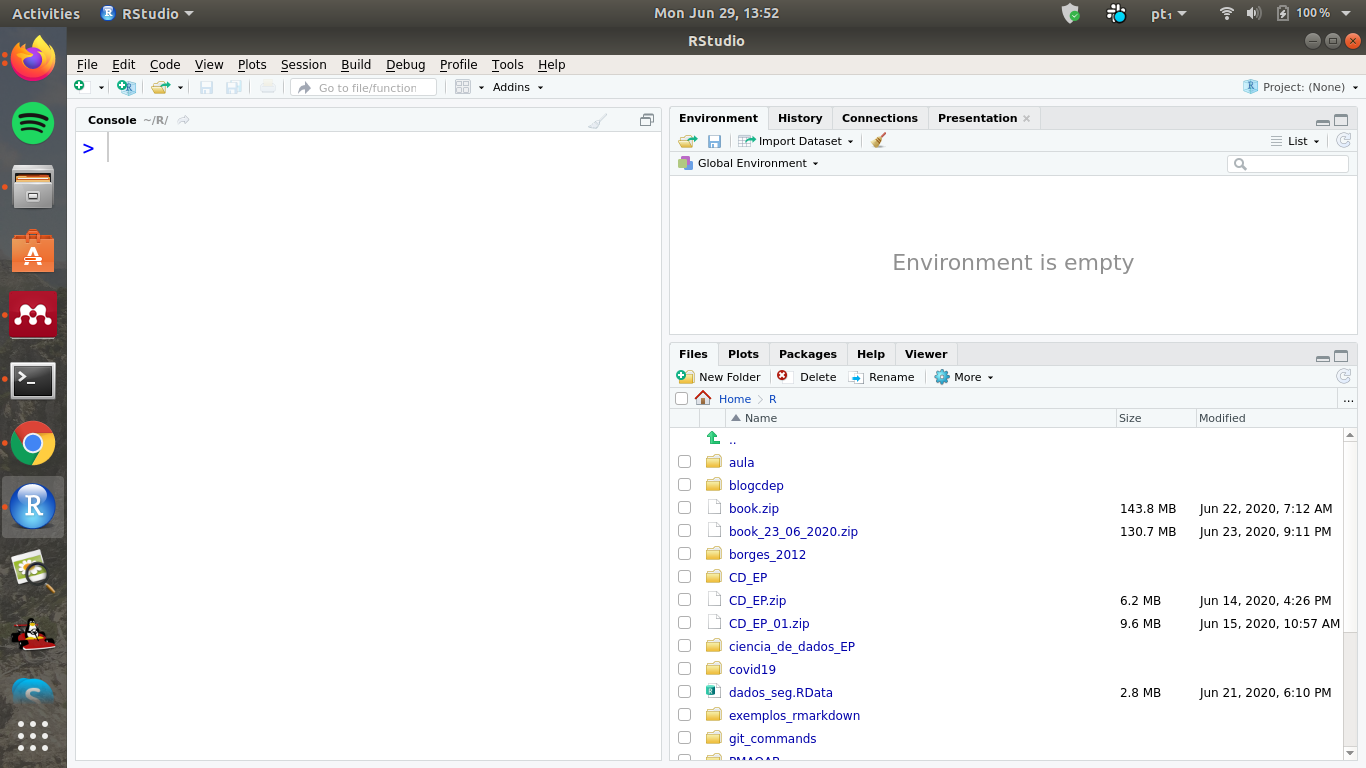
\includegraphics{fig/open_Rstudio.png}
\caption{Opção de instalação pelo modo gráfico}
\end{figure}

\begin{enumerate}
\def\labelenumi{\arabic{enumi}.}
\setcounter{enumi}{1}
\tightlist
\item
  Selecoine a aba de instalação \emph{Packages} e clique em \textbf{install},
\end{enumerate}

\begin{figure}
\centering
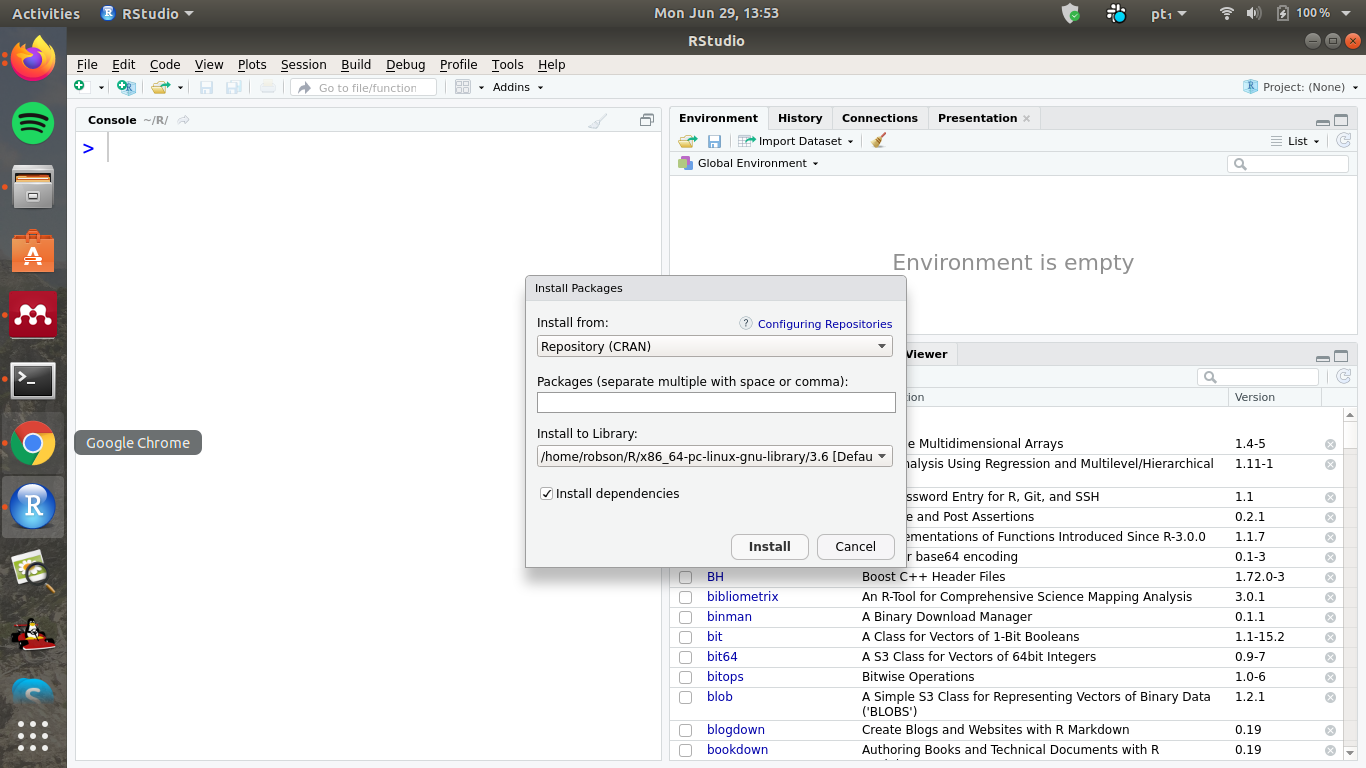
\includegraphics{fig/install_packages_rstudio_visual.png}
\caption{Selecoinar aba de instalação \emph{Packages - Click em install}}
\end{figure}

\begin{enumerate}
\def\labelenumi{\arabic{enumi}.}
\setcounter{enumi}{2}
\tightlist
\item
  No ambiente de busca da interface instalação pesquise
  por \emph{bookdown}, selecione o pacote e clique em \emph{install},
\end{enumerate}

\begin{figure}
\centering
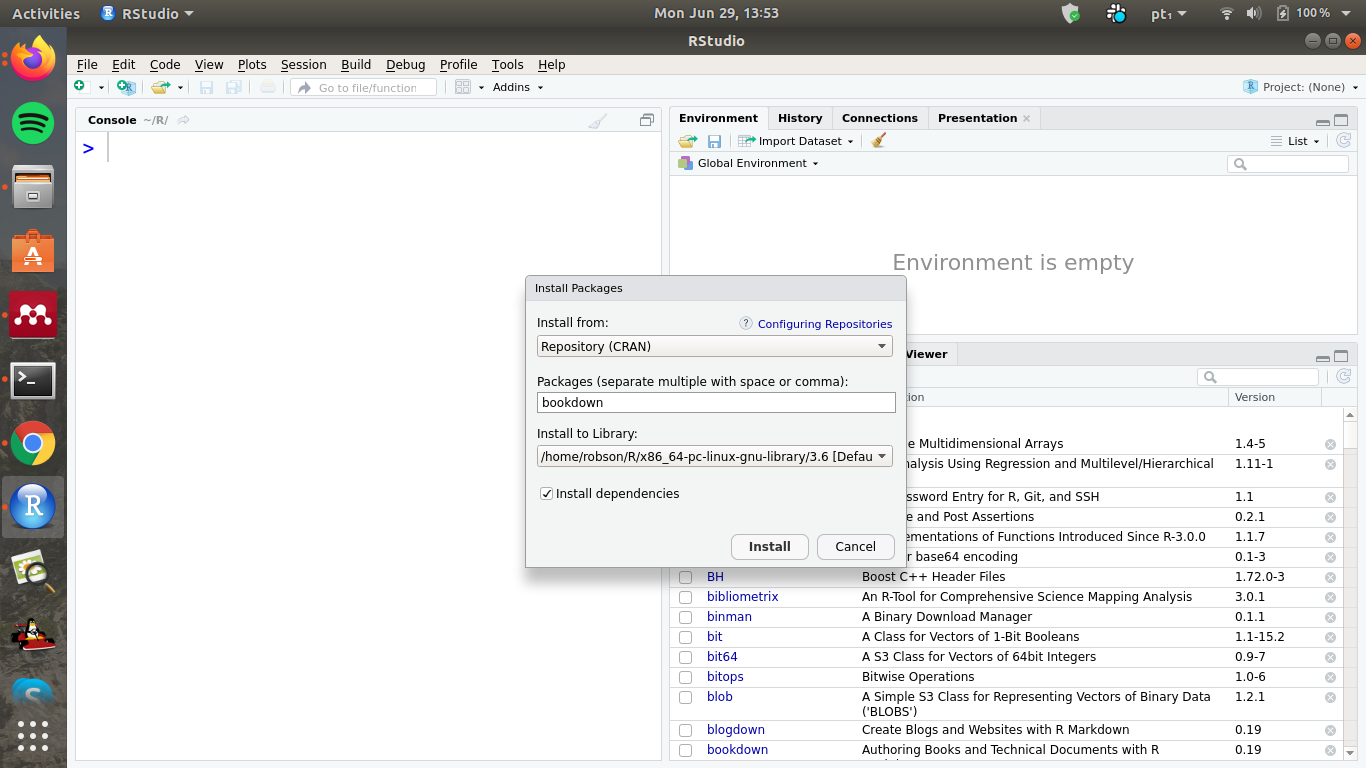
\includegraphics{fig/install_packages_rstudio_visual_bookdown.png}
\caption{\emph{Pesquisar por bookdown e clicar em install}}
\end{figure}

\begin{enumerate}
\def\labelenumi{\arabic{enumi}.}
\setcounter{enumi}{3}
\item
  Finalmente, o código será instalado,
  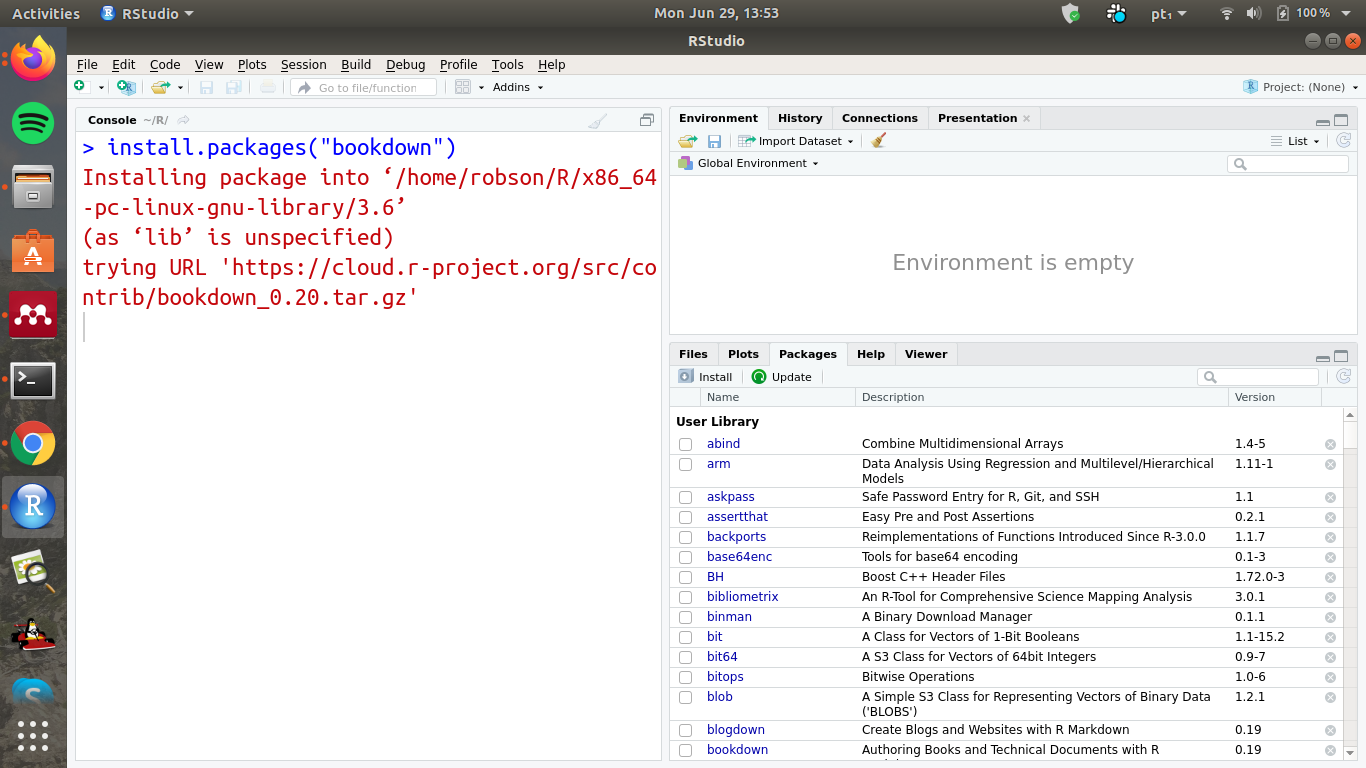
\includegraphics{fig/install_packages_rstudio_visual_bookdown_run.png}
\item
  Ainda é necessário carregá-lo na seção de uso, novamente na aba \emph{Packages} pesquise por \emph{bookdown}
  e selecione o pacote, o que será suficiente para
  carregá-lo,
\end{enumerate}

\begin{figure}
\centering
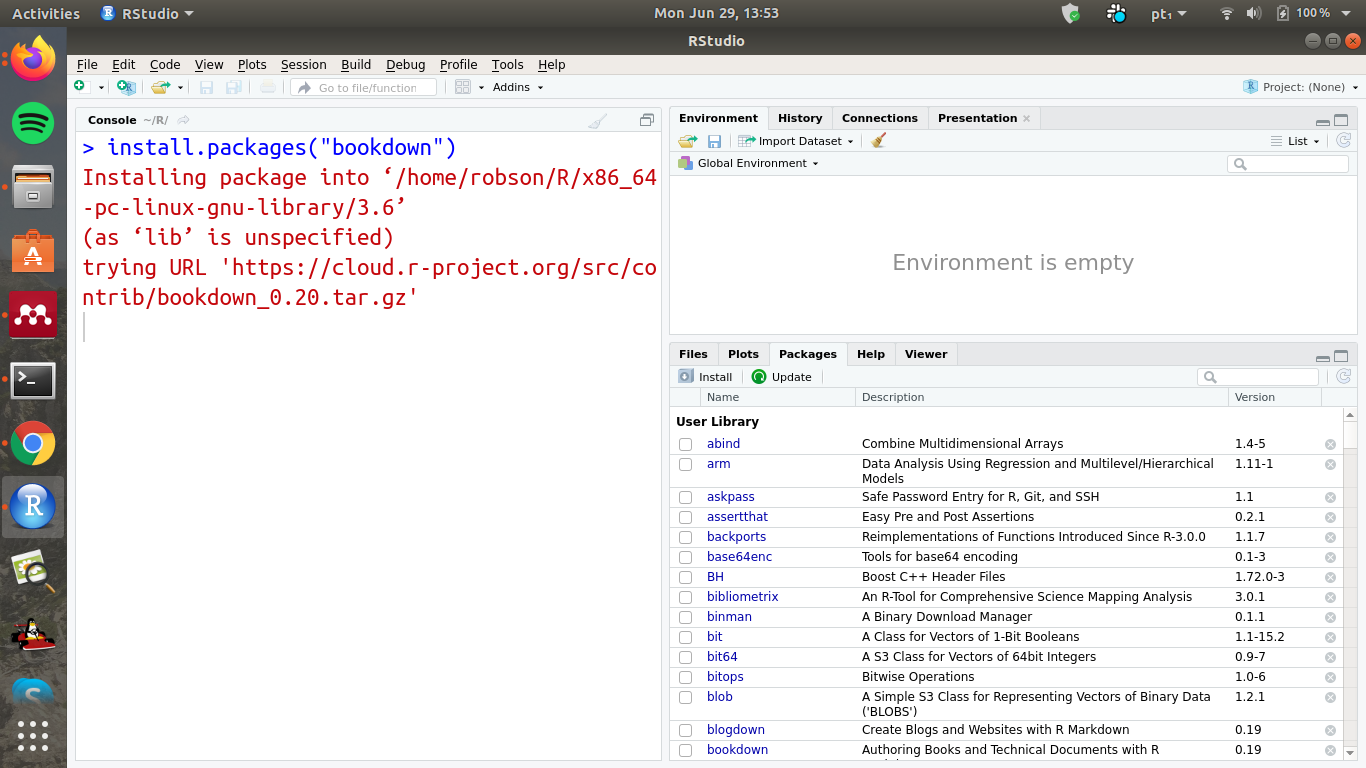
\includegraphics{fig/install_packages_rstudio_visual_bookdown_run.png}
\caption{Carregar a biblioteca bookdown na aba Package}
\end{figure}

\begin{Shaded}
\begin{Highlighting}[]
\KeywordTok{install.packages}\NormalTok{(}\StringTok{"bookdown"}\NormalTok{)}
\CommentTok{# or the development version}
\CommentTok{# devtools::install_github("rstudio/bookdown")}
\KeywordTok{library}\NormalTok{(}\StringTok{"bookdown"}\NormalTok{)}
\end{Highlighting}
\end{Shaded}

Deve-se lembrar que para cada arquivo \emph{.Rmd}
só pode ter um capítulo sendo definido pelo primeiro nível
por \texttt{\#}.

Para compilar este exemplo para PDF, é necessário
o pacote XeLaTeX. É recomendável
instalar o TinyTeX (que inclui o XeLaTeX): \url{https://yihui.org/tinytex/}.

Nos próximos capítulos serão apresentados outros
detalhes sobre instalação e configuração.

\hypertarget{intro}{%
\chapter{Introdução}\label{intro}}

A primeira palavra que devemos pensar
ao encarar um curso de ferramentas de
escrita de textos é \emph{oportunidade}.

Quando pensamos em texto simples e rápidos,
podemos naturalmente usar ferramentas como
WYSIWYG (\emph{What You See Is What You Get})
como \textbf{LibreOffice Writer} ou
\textbf{Microsof Office Word}. Entretanto,
trabalhar com textos longos, como relatórios,
trabalhos de conclusão de curso (TCC),
dissertações ou teses pode exigir
recursos mais avançados como LaTeX.

\hypertarget{criauxe7uxe3o-do-projeto-do-livro}{%
\section{Criação do projeto do livro}\label{criauxe7uxe3o-do-projeto-do-livro}}

Faremos uso mais uma vez de recursos
gráficos da interface do \emph{Rstudio}
para a criação do projeto do livro.
Este material foi prepara utilizando
a estrutura mínima disponibilizada pelo
\emph{template} do pacote \emph{bookdown}.
As etapas a seguir serão o suficiente
para entender a criação e uso desse \emph{template}:

\begin{enumerate}
\def\labelenumi{\arabic{enumi}.}
\tightlist
\item
  Após a instalação e carregamento da biblioteca
  \emph{bookdown}, podemos utilizar o \emph{template},
  primeiro devemos clicar no canto superior direito em \emph{projetos} como:
\end{enumerate}

\begin{figure}
\centering
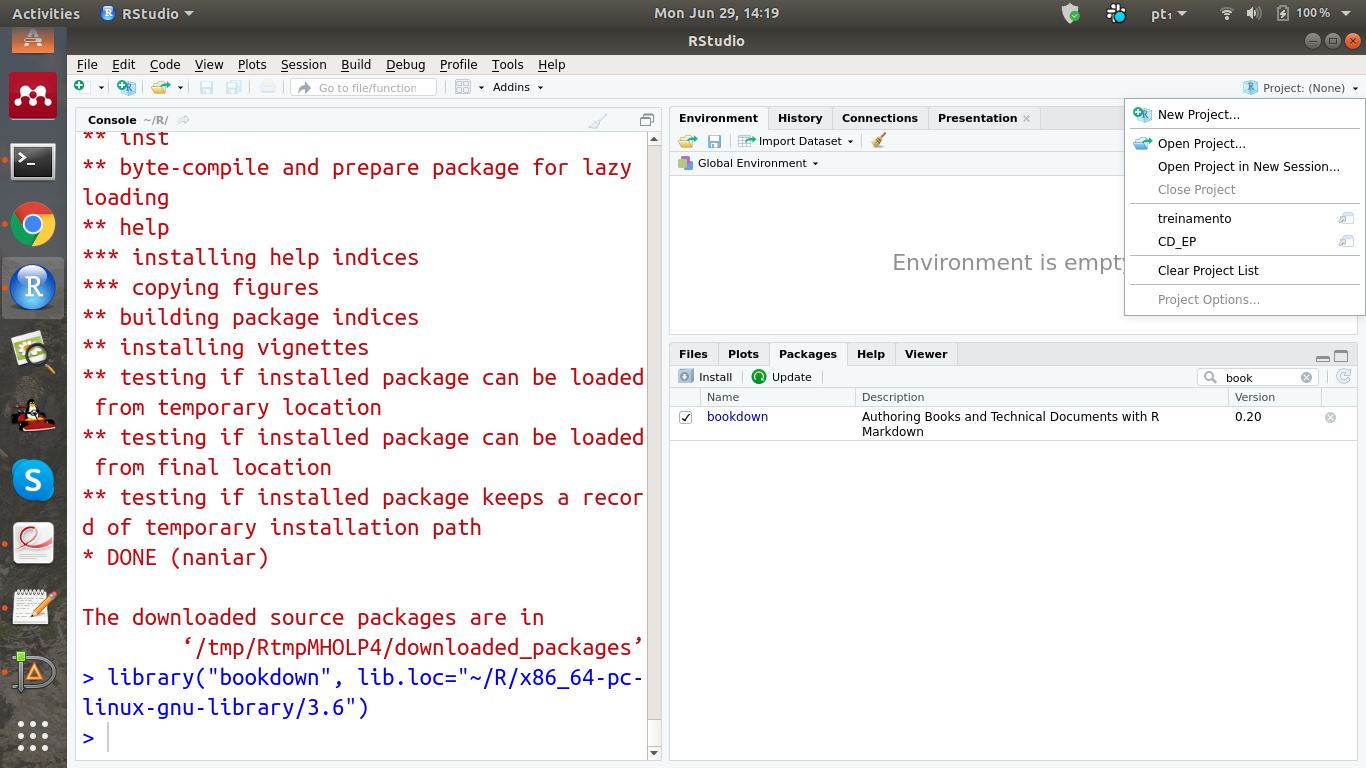
\includegraphics{fig/rstudio_select_new_Project.png}
\caption{Criação de um novo projeto de livro}
\end{figure}

\begin{enumerate}
\def\labelenumi{\arabic{enumi}.}
\setcounter{enumi}{1}
\tightlist
\item
  Em seguida, selecionar \emph{New Directory}:
\end{enumerate}

\begin{figure}
\centering
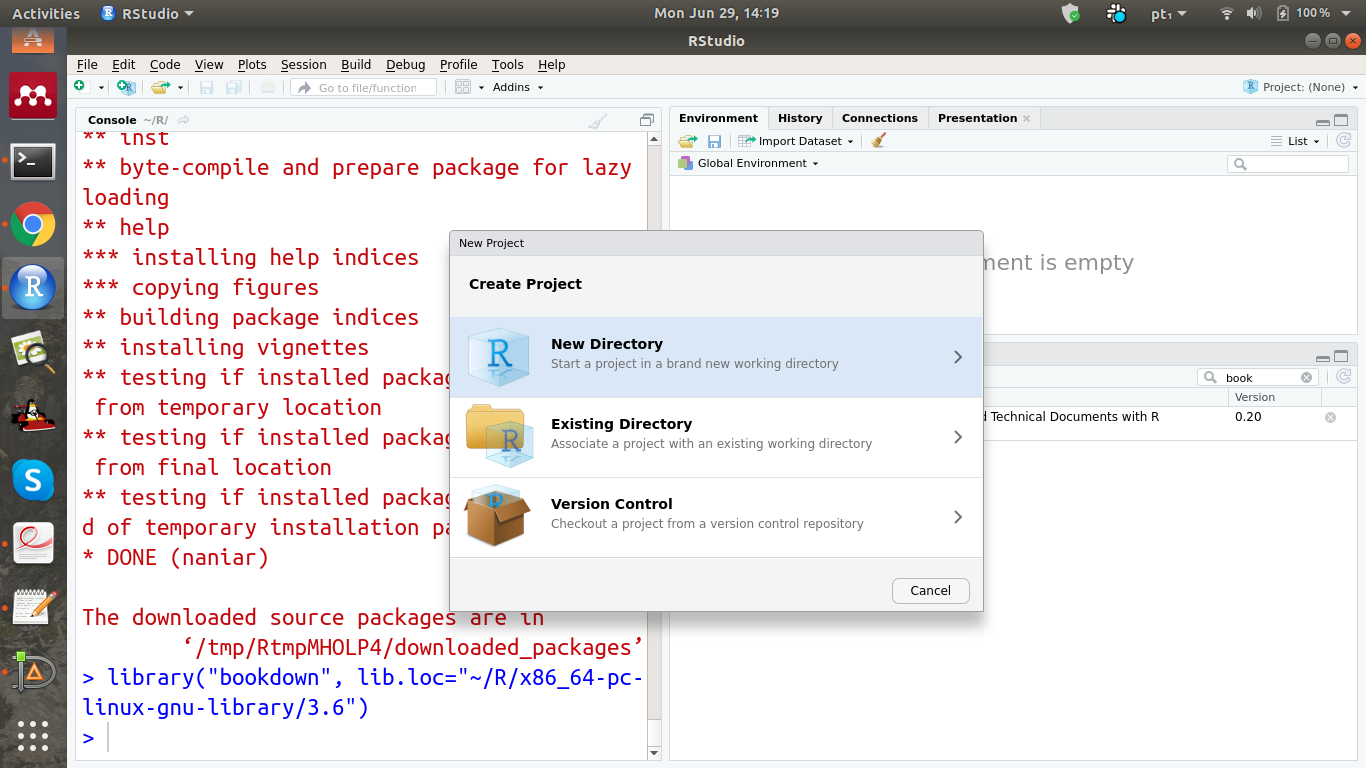
\includegraphics{fig/select_new_directory.png}
\caption{Selecionar a criação de um novo diretório}
\end{figure}

\begin{enumerate}
\def\labelenumi{\arabic{enumi}.}
\setcounter{enumi}{2}
\tightlist
\item
  Selecionar \emph{Book Project with bookdown}
\end{enumerate}

\begin{figure}
\centering
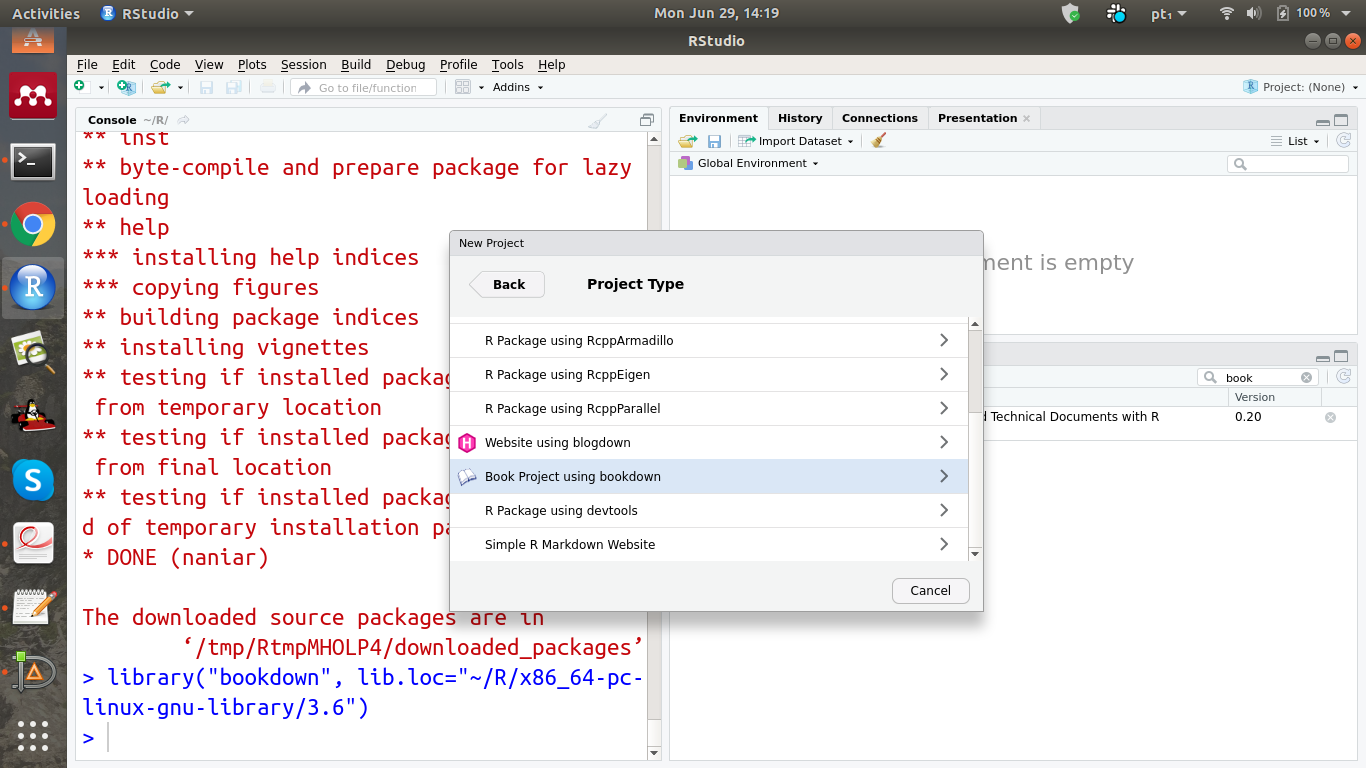
\includegraphics{fig/select_Book_Project_with_bookdown.png}
\caption{Seleção da opção de projeto de livro com pacote bookdown}
\end{figure}

\begin{enumerate}
\def\labelenumi{\arabic{enumi}.}
\setcounter{enumi}{3}
\tightlist
\item
  Em seguida o template com a versão mínima será
  disponibilizado por meio de uma pasta com o nome escolhido na etapa anterior.
\end{enumerate}

\begin{figure}
\centering
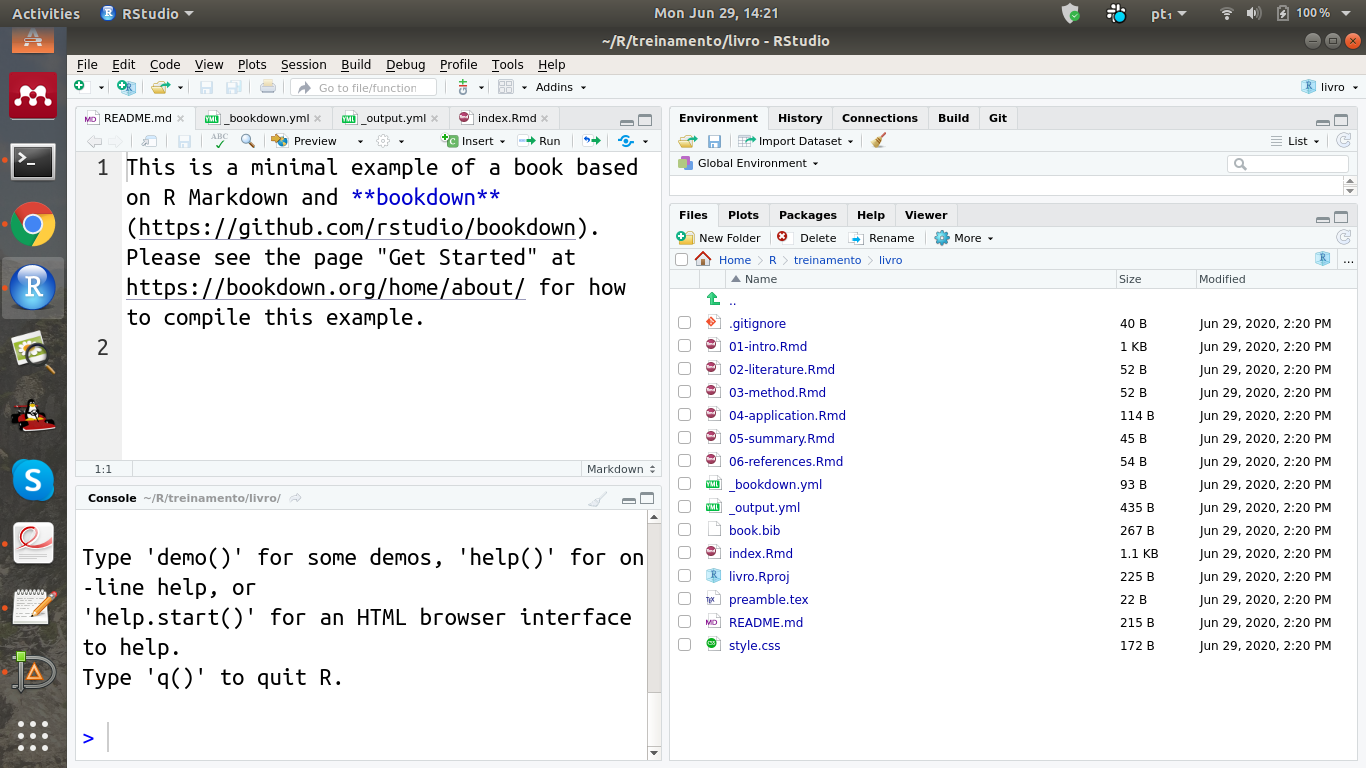
\includegraphics{fig/outra.png}
\caption{Seleção da opção de projeto de livro com pacote bookdown}
\end{figure}

Na lista apresentada acima são identificados
arquivos com as seguintes extensões:

\begin{itemize}
\tightlist
\item
  \textbf{.Rmd}
\item
  \textbf{.bib}
\item
  \textbf{.yml}
\item
  \textbf{.tex}
\item
  \textbf{.css}
\end{itemize}

Aqueles arquivos cuja a extensão é \emph{.Rmd}
são utilizados para a escrita dos
conteúdos do livro em R Markdown. Entretanto,
entre eles
há um especial, \emph{index.Rmd}, que constrói
a página principal, por meio de
comandos \textbf{yml}. Algumas configurações
são reservadas em dois arquivos com extensão
\textbf{.yml}. Sendo o arquivo \_bookdown.yml para
configurações gerais que serão úteis para quaisquer
tipo de documento de saída, por exemplo, a definição
se o título de cada capítulo será chamado de
\textbf{Chapter } ou \textbf{Capítulo }, especialmente
para este treinamento fizemos esta alteração. Enquanto
que para o arquivo *\_output.yml* são apresentadas
configurações especiais para cada tipo de saída,
como \emph{bookdown::gitbook}, \emph{bookdown::pdf\_book:} ou
\emph{bookdown::epub\_book:}. Especialmente para o
caso do \emph{gitbook} é necessário a existência do arquivo
\emph{style.css} para algumas configurações. Já o arquivo
\emph{book.bib} é uma estrutura especial do pacote \emph{bibtex}
do LaTeX e contem as informações de artigos que serão citados.

\hypertarget{literatura-e-bibtex}{%
\chapter{Literatura e bibtex}\label{literatura-e-bibtex}}

O foco deste capítulo está numa das
principais potencialidades do LaTeX
utilizas pelo R Markdown a capacidade
de citar os documentos adequadamente
organizados num arquivo \emph{.bib},
especialmente neste exemplo aproveitamos
o arquivo gerado pela estrutura mínima
\emph{bookdown}.

Para esta etapa aproveitaremos como exemplo
os artigos do projeto organizados na
plataforma Mendeley, seguindo os
seguintes passos:

\begin{enumerate}
\def\labelenumi{\arabic{enumi}.}
\tightlist
\item
  Abrir Medeley Desktop;
\item
  Abrir pasta do grupo nomeada por CDnaEP;
\item
  Selecionar os artigos que pretende citar no seu documento;
\item
  Clicar com o botão direito do mouse, selecionar \emph{Copy as} e em seguida \emph{BibTex entry}.
\item
  Abrir o arquivo \emph{book.bib} e colar os metadados
  dos artigos na última linha do arquivo depois da
  última chave \textbf{\}}.
\item
  Em seguida, salve e feche o arquivo \emph{book.bib}.
\end{enumerate}

As figuras a seguir estão de acordo com a sequência acima apresentada:

\begin{figure}
\centering
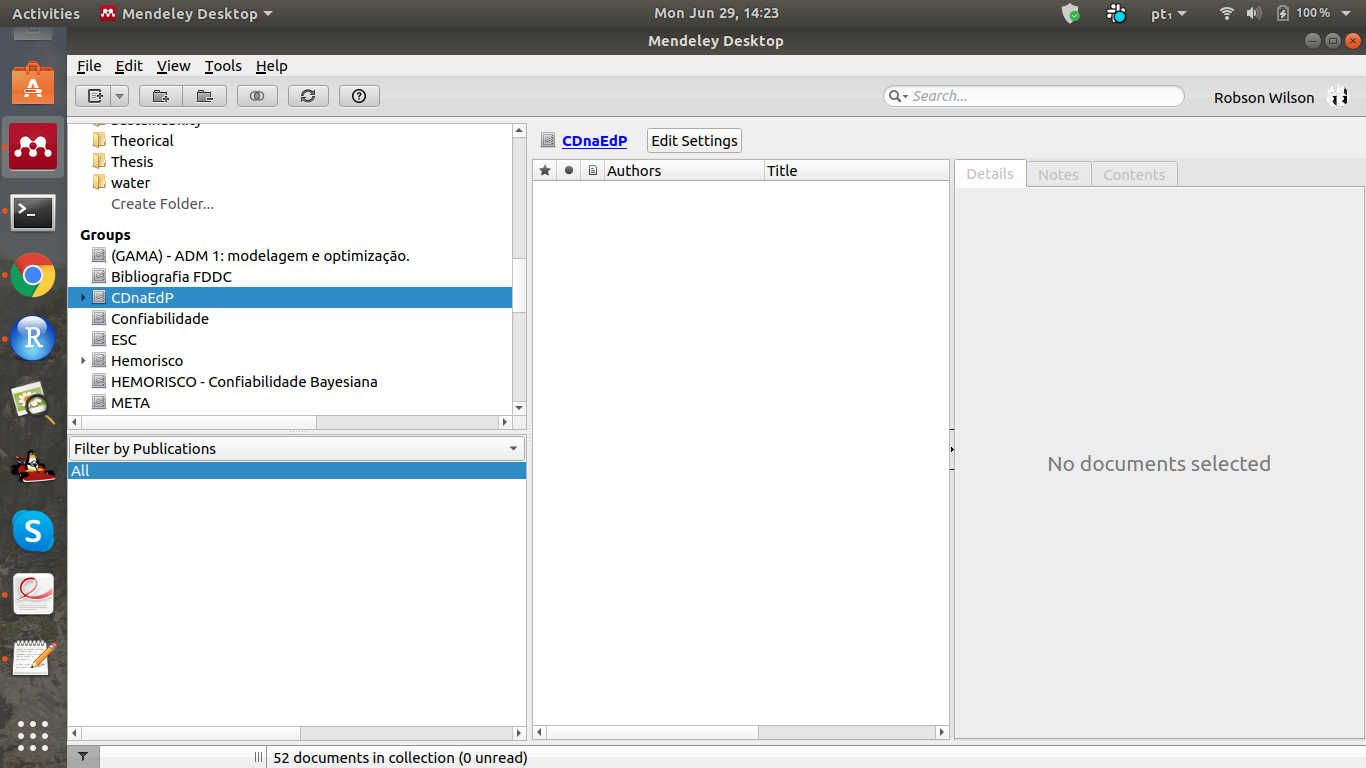
\includegraphics{fig/open_mendeley.png}
\caption{Abrir Medeley Desktop e selecionar pasta CDna EP}
\end{figure}

\begin{figure}
\centering
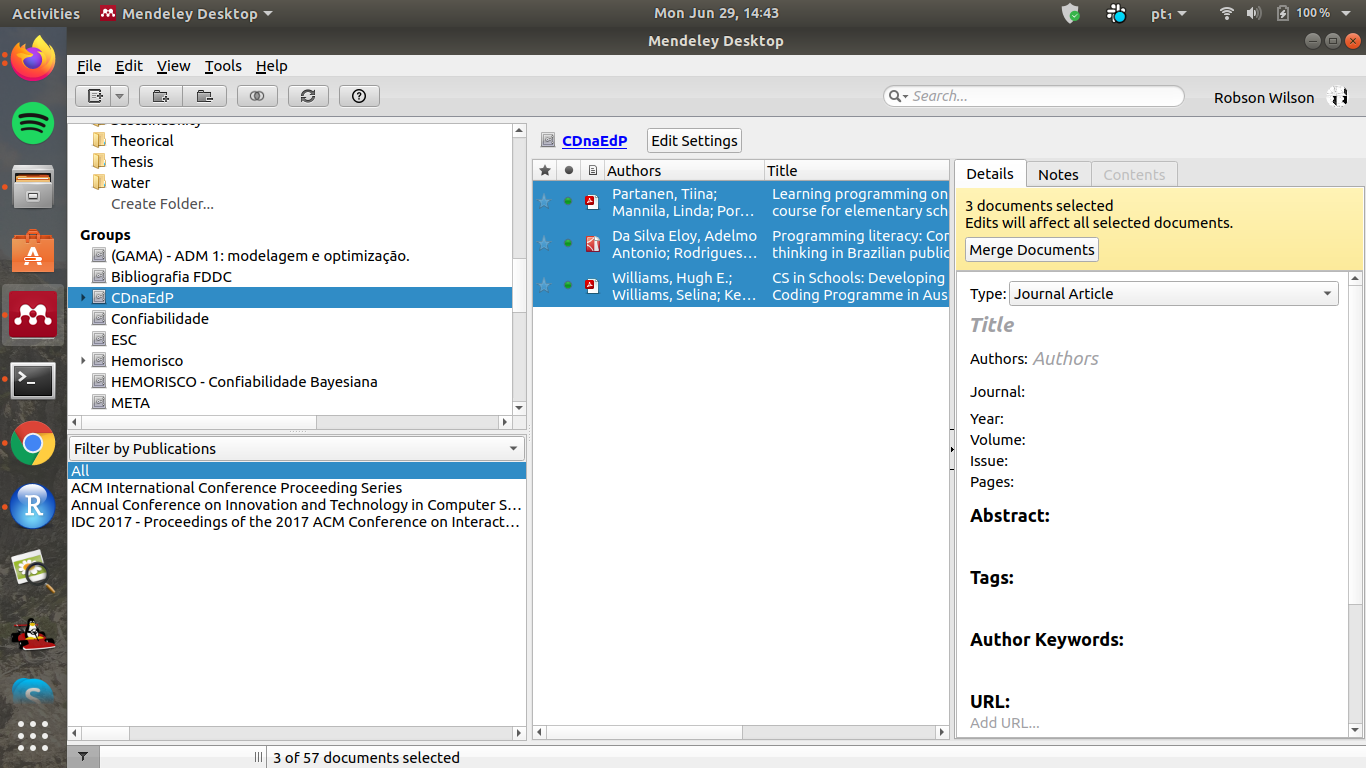
\includegraphics{fig/mendeley_select_CDnaEP_paper_list.png}
\caption{Selecionar artigos para citação}
\end{figure}

\begin{figure}
\centering
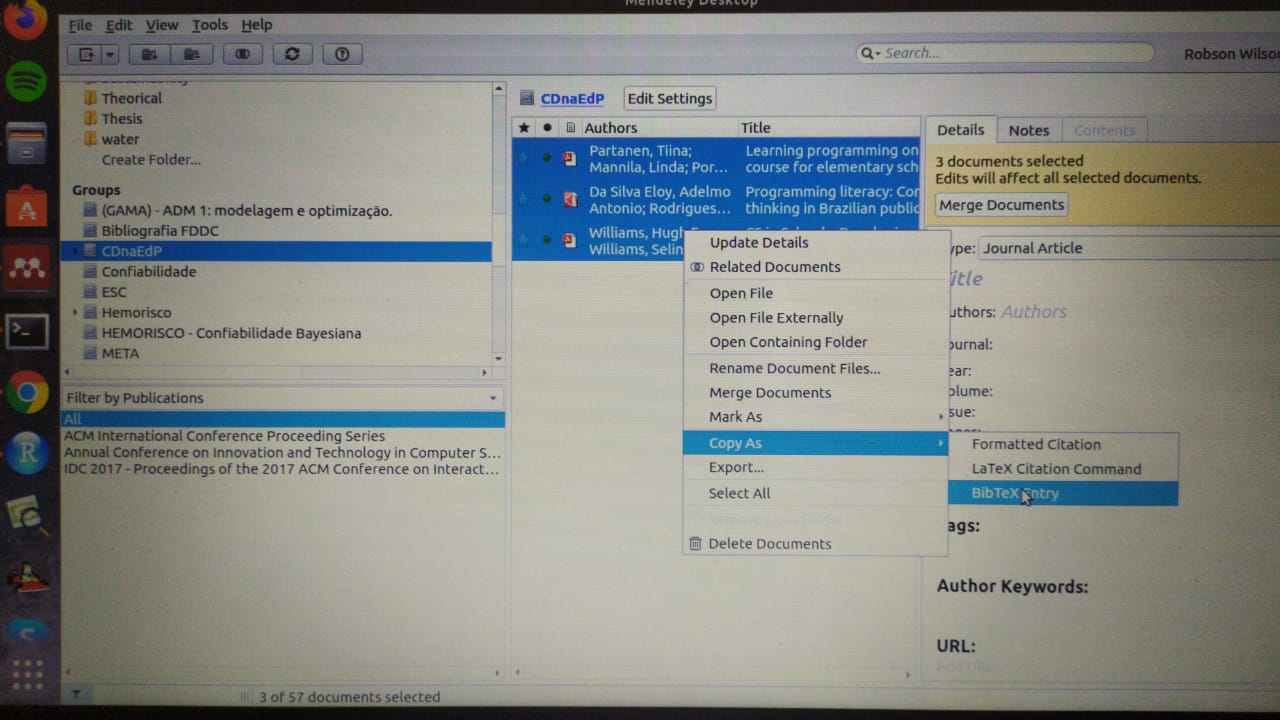
\includegraphics{fig/mendeley_copy_bibtex_entry.jpeg}
\caption{Copiar metadados no formato de entrada do bibtex}
\end{figure}

Uma informação importante para quem ainda não
é familiarizado com LaTeX é o fato
da primeira informação dos metados
de um artigo dentro do arquivo \emph{.bib}
ser a \emph{label}, a informação que será
usada para citações ao longo do documento.

\begin{figure}
\centering
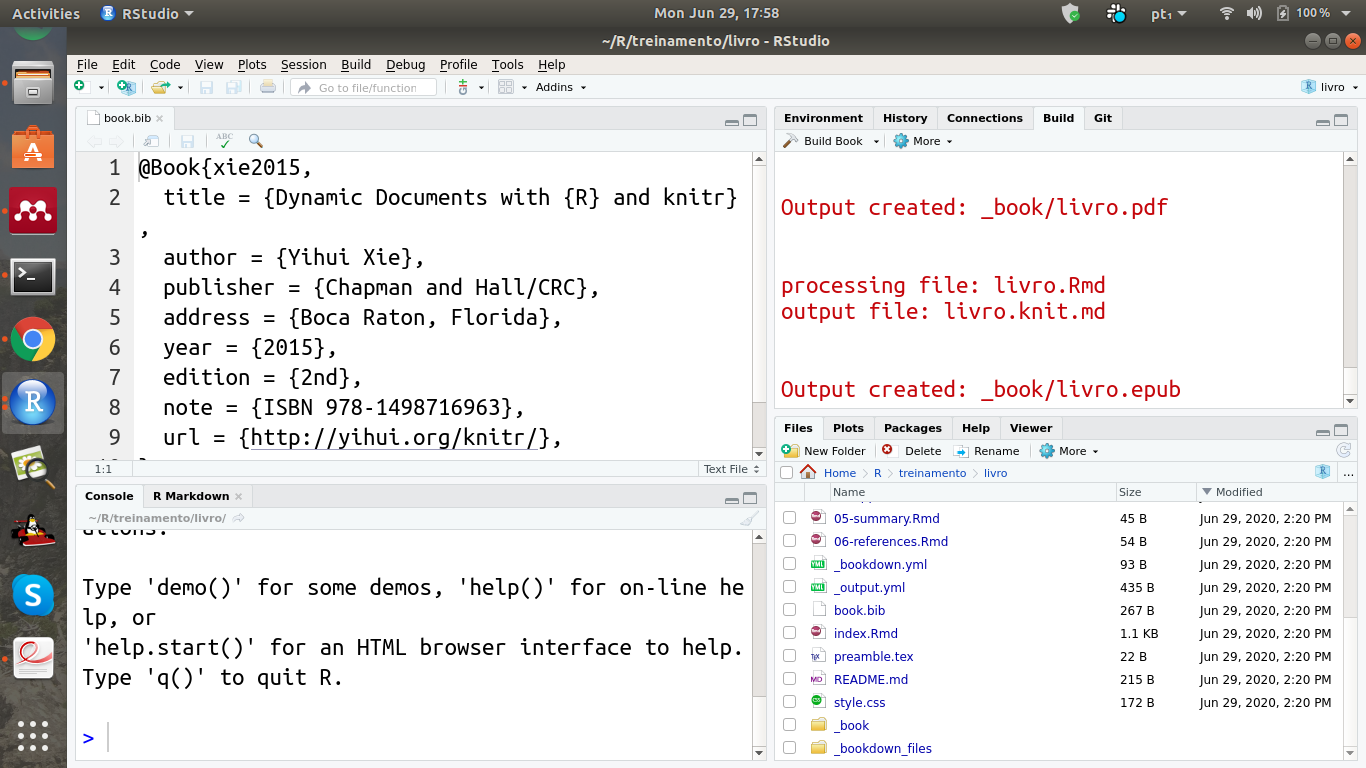
\includegraphics{fig/rstudio_open_bookbib_first.png}
\caption{Identificação da \emph{label} do livro do (\citep{xie2015})}
\end{figure}

\begin{figure}
\centering
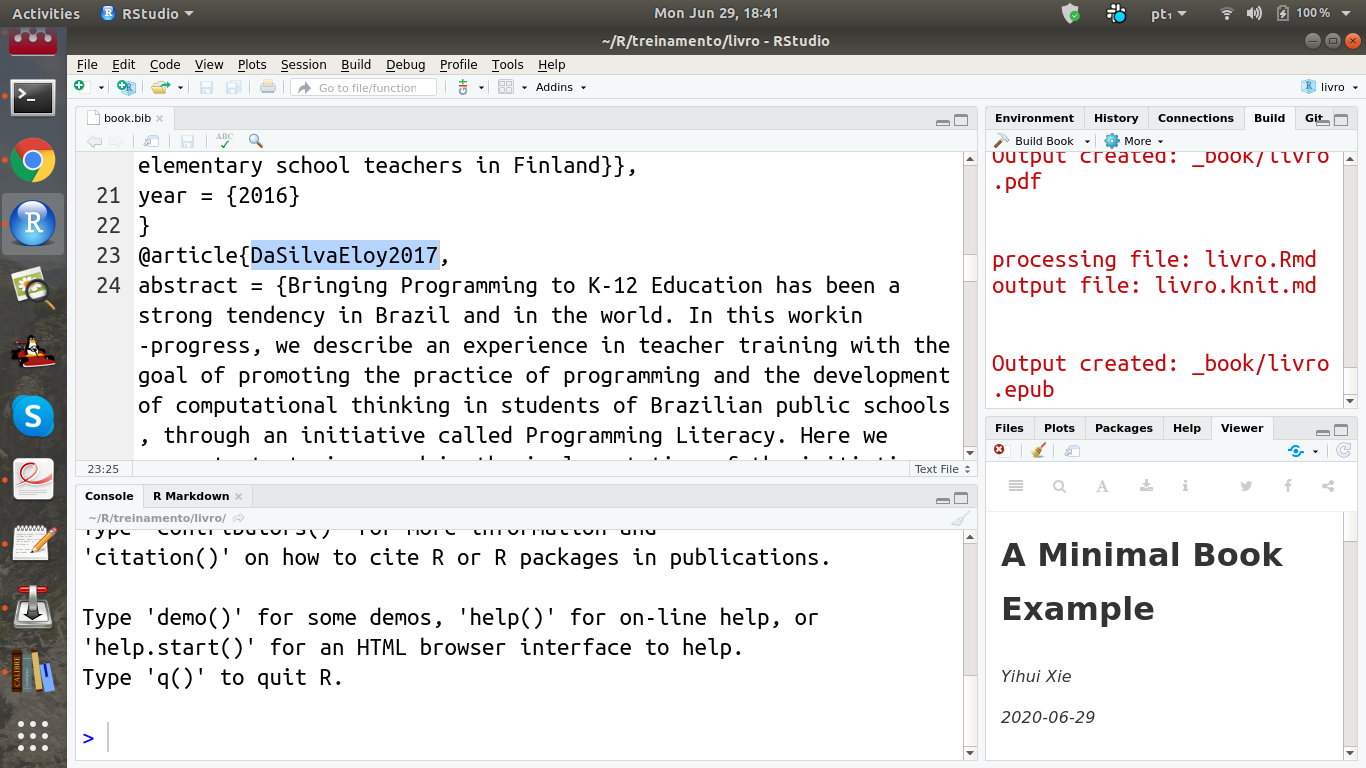
\includegraphics{fig/rstudio_open_bookbib_second.png}
\caption{Identificação da \emph{label} de cada artigo (\citep{DaSilvaEloy2017})}
\end{figure}

\begin{figure}
\centering
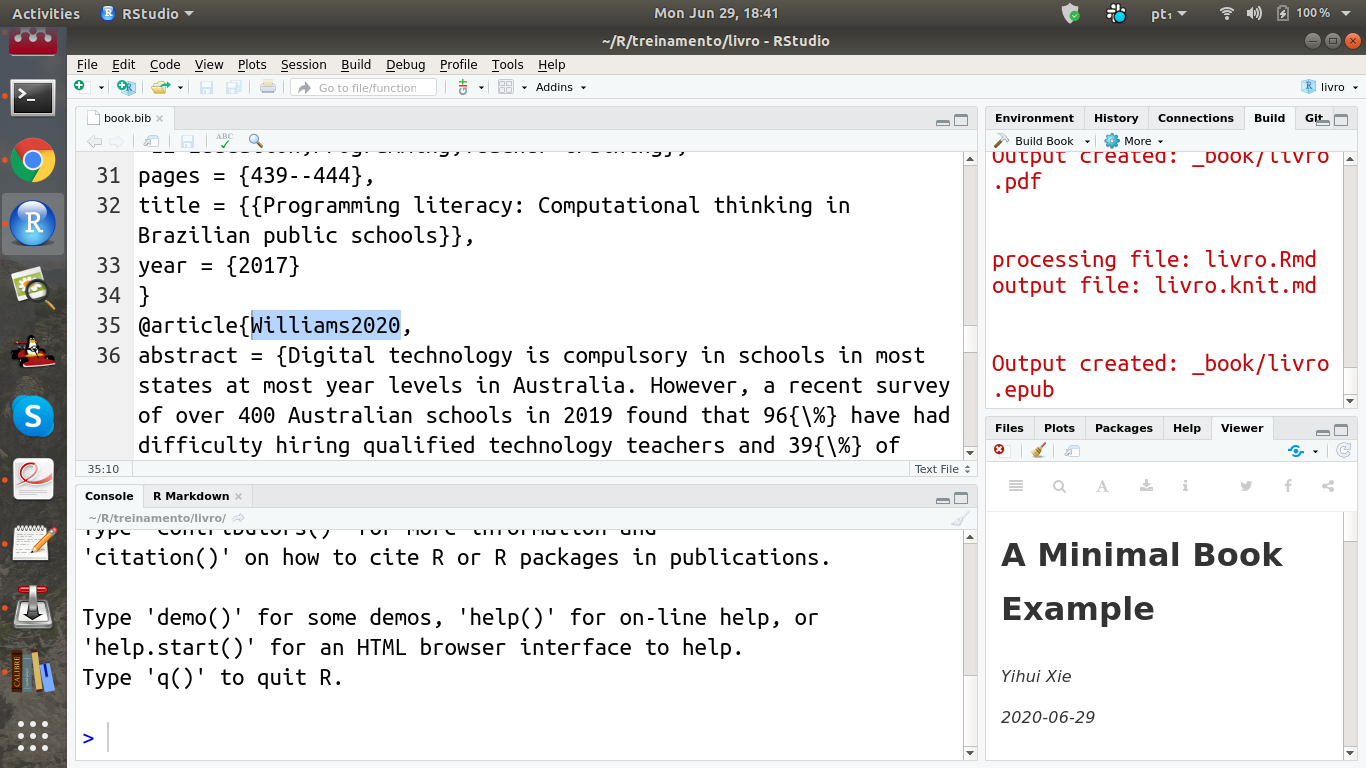
\includegraphics{fig/rstudio_open_bookbib_third.png}
\caption{Identificação da \emph{label} de cada artigo (\citep{Williams2020})}
\end{figure}

Nas subseções a seguir mostramos como citar alguns desses trabalhos.

\hypertarget{exemplo-de-citauxe7uxe3o-simples}{%
\section{Exemplo de citação simples}\label{exemplo-de-citauxe7uxe3o-simples}}

Vamos considerar a citação do artigo \citep{Partanen2016}.

\hypertarget{citauxe7uxf5es-de-dois-ou-mais-artigos}{%
\section{Citações de dois ou mais artigos}\label{citauxe7uxf5es-de-dois-ou-mais-artigos}}

Agora incluiremos mais duas citações \citep[\citet{Williams2020}]{DaSilvaEloy2017}.

\hypertarget{capitulo-3}{%
\chapter{Visualização e Análise gráfica na Ciência de dados}\label{capitulo-3}}

O capítulo \ref{capitulo-2} apresenta a tabela como uma forma poderosa para estruturar e visualizar informações. No entanto, quando trabalhamos com enormes tabelas com uma imensa quantidade de linhas e colunas se torna difícil interpretar suas informações, não importa o quão organizadas elas estejam. Às vezes, é muito mais fácil interpretar essas informações através de gráficos, conteúdo que será explorado no decorrer deste capítulo.

A construção e visualização gráfica é de extrema importância na área de ciência de dados, pois é a partir de um bom gráfico que se torna possível extrair ideias, hipóteses ou até conclusões a respeito de um tema. A importância desse tipo de análise pode ser expressa por um ditado popular bastante conhecido: ``Uma imagem vale por mil palavras''.

Para demonstrar os diferentes tipos de gráficos que você pode encontrar nesta área, serão utilizadas duas bases de dados primordiais para exemplificar os conceitos deste capítulo: os microdados do Exame Nacional do Ensino Médio (ENEM) de 2018 para os estudantes da cidade de Salvador (Bahia) e diversas informações sobre o turismo na capital bahiana. Os microdados do ENEM são publicados pelo Instituto Nacional de Estudos e Pesquisas Educacionais Anísio Teixeira (INEP) em seu site. Já as informações sobre o turismo advém de diversas fontes ligadas ao governo do estado da Bahia, mais precisamente a Secretaria de Turismo do Estado da Bahia (SETUR).

\hypertarget{gruxe1fico-de-barra}{%
\section{Gráfico de barra}\label{gruxe1fico-de-barra}}

O \textbf{Gráfico de barras} é uma forma bastante comum de visualização na área de ciência de dados sendo bastante utilizado para expressar noções de variáveis categóricas.

Seguindo uma definição mais formal, trata-se da exibição de barras, igualmente espaçadas e largas, para cada categoria. O comprimento, ou seja, o tamanho de cada barra será proporcional à \textbf{frequência} desta categoria. Será através da interpretação das frequências dispostas que perguntas como ``qual a categoria mais dominante desta variável?'' ou ``qual categoria apresenta uma menor quantidade?'' podem ser respondidas. Como exemplo é apresentado o gráfico abaixo:

\begin{figure}

{\centering 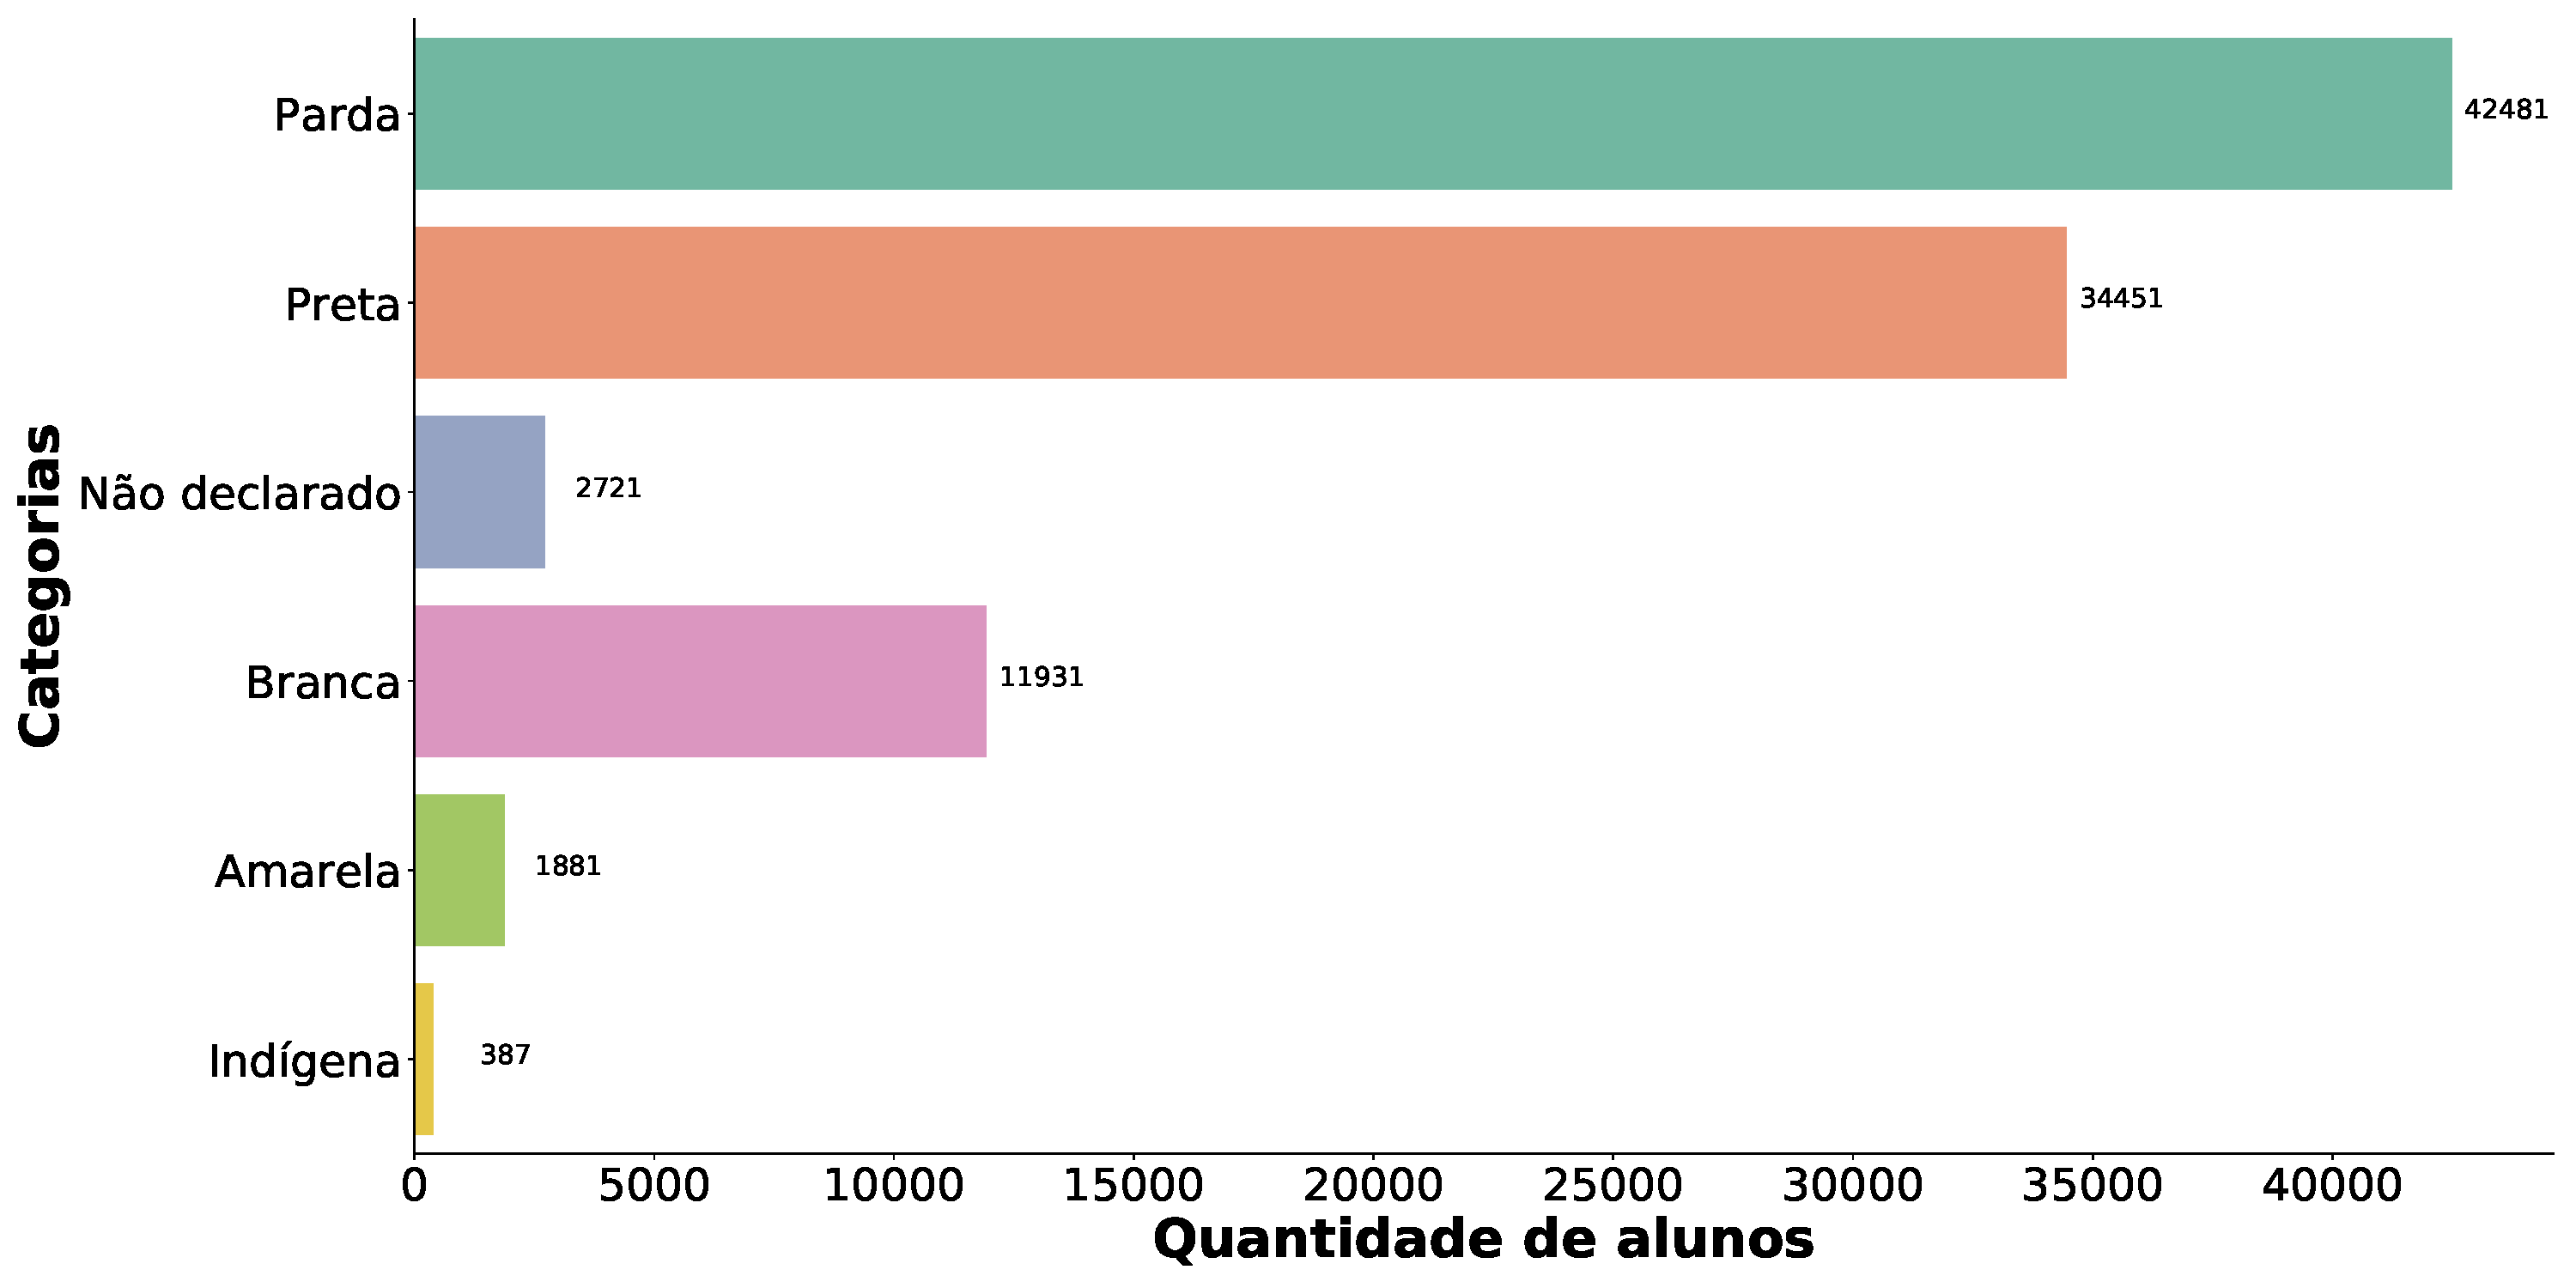
\includegraphics[width=0.9\linewidth]{livro_files/figure-latex/fig31-1} 

}

\caption{Distinção de estudantes por cor/raça da cidade de Salvador inscritos no ENEM 2018}\label{fig:fig31}
\end{figure}

A \texttt{fig31} apresenta a distinção de estudantes por cor/raça inscritos no ENEM 2018 na cidade de Salvador (BA), onde os valores a direita das barras indicam a quantidade de alunos pertencentes aquela categoria. Através da análise deste gráfico é possível responder as perguntas apresentadas anteriormente como:
- ``Qual a categoria mais dominante nesta variável?'' A categoria \texttt{Parda} domina em maior quantidade. Ou seja, em Salvador existem mais estudantes auto declarados pardos.
- ``Qual a categoria apresenta uma menor quantidade?'' A categoria \texttt{Indígena} apresenta uma baixa representatividade.

Note como uma visualização gráfica é melhor em comparação a uma tabela para a mesma informação:

\begin{verbatim}
## 0     Parda
## 1     Preta
## 2     Preta
## 3     Parda
## 4     Preta
##       ...  
## 95    Parda
## 96    Preta
## 97    Parda
## 98    Preta
## 99    Parda
## Name: TP_COR_RACA, Length: 100, dtype: object
\end{verbatim}

Ao invés do trabalho repetitivo de contar na tabela quantos estudantes estão em cada categoria, através de uma linguagem de programação com alguns comandos isso é realizado de forma automática!

Apesar do gráfico anterior apresentar informações interessantes, sua construção pode ser aprimorada ainda mais e é isso o que a figura seguinte irá trazer:

\begin{figure}

{\centering 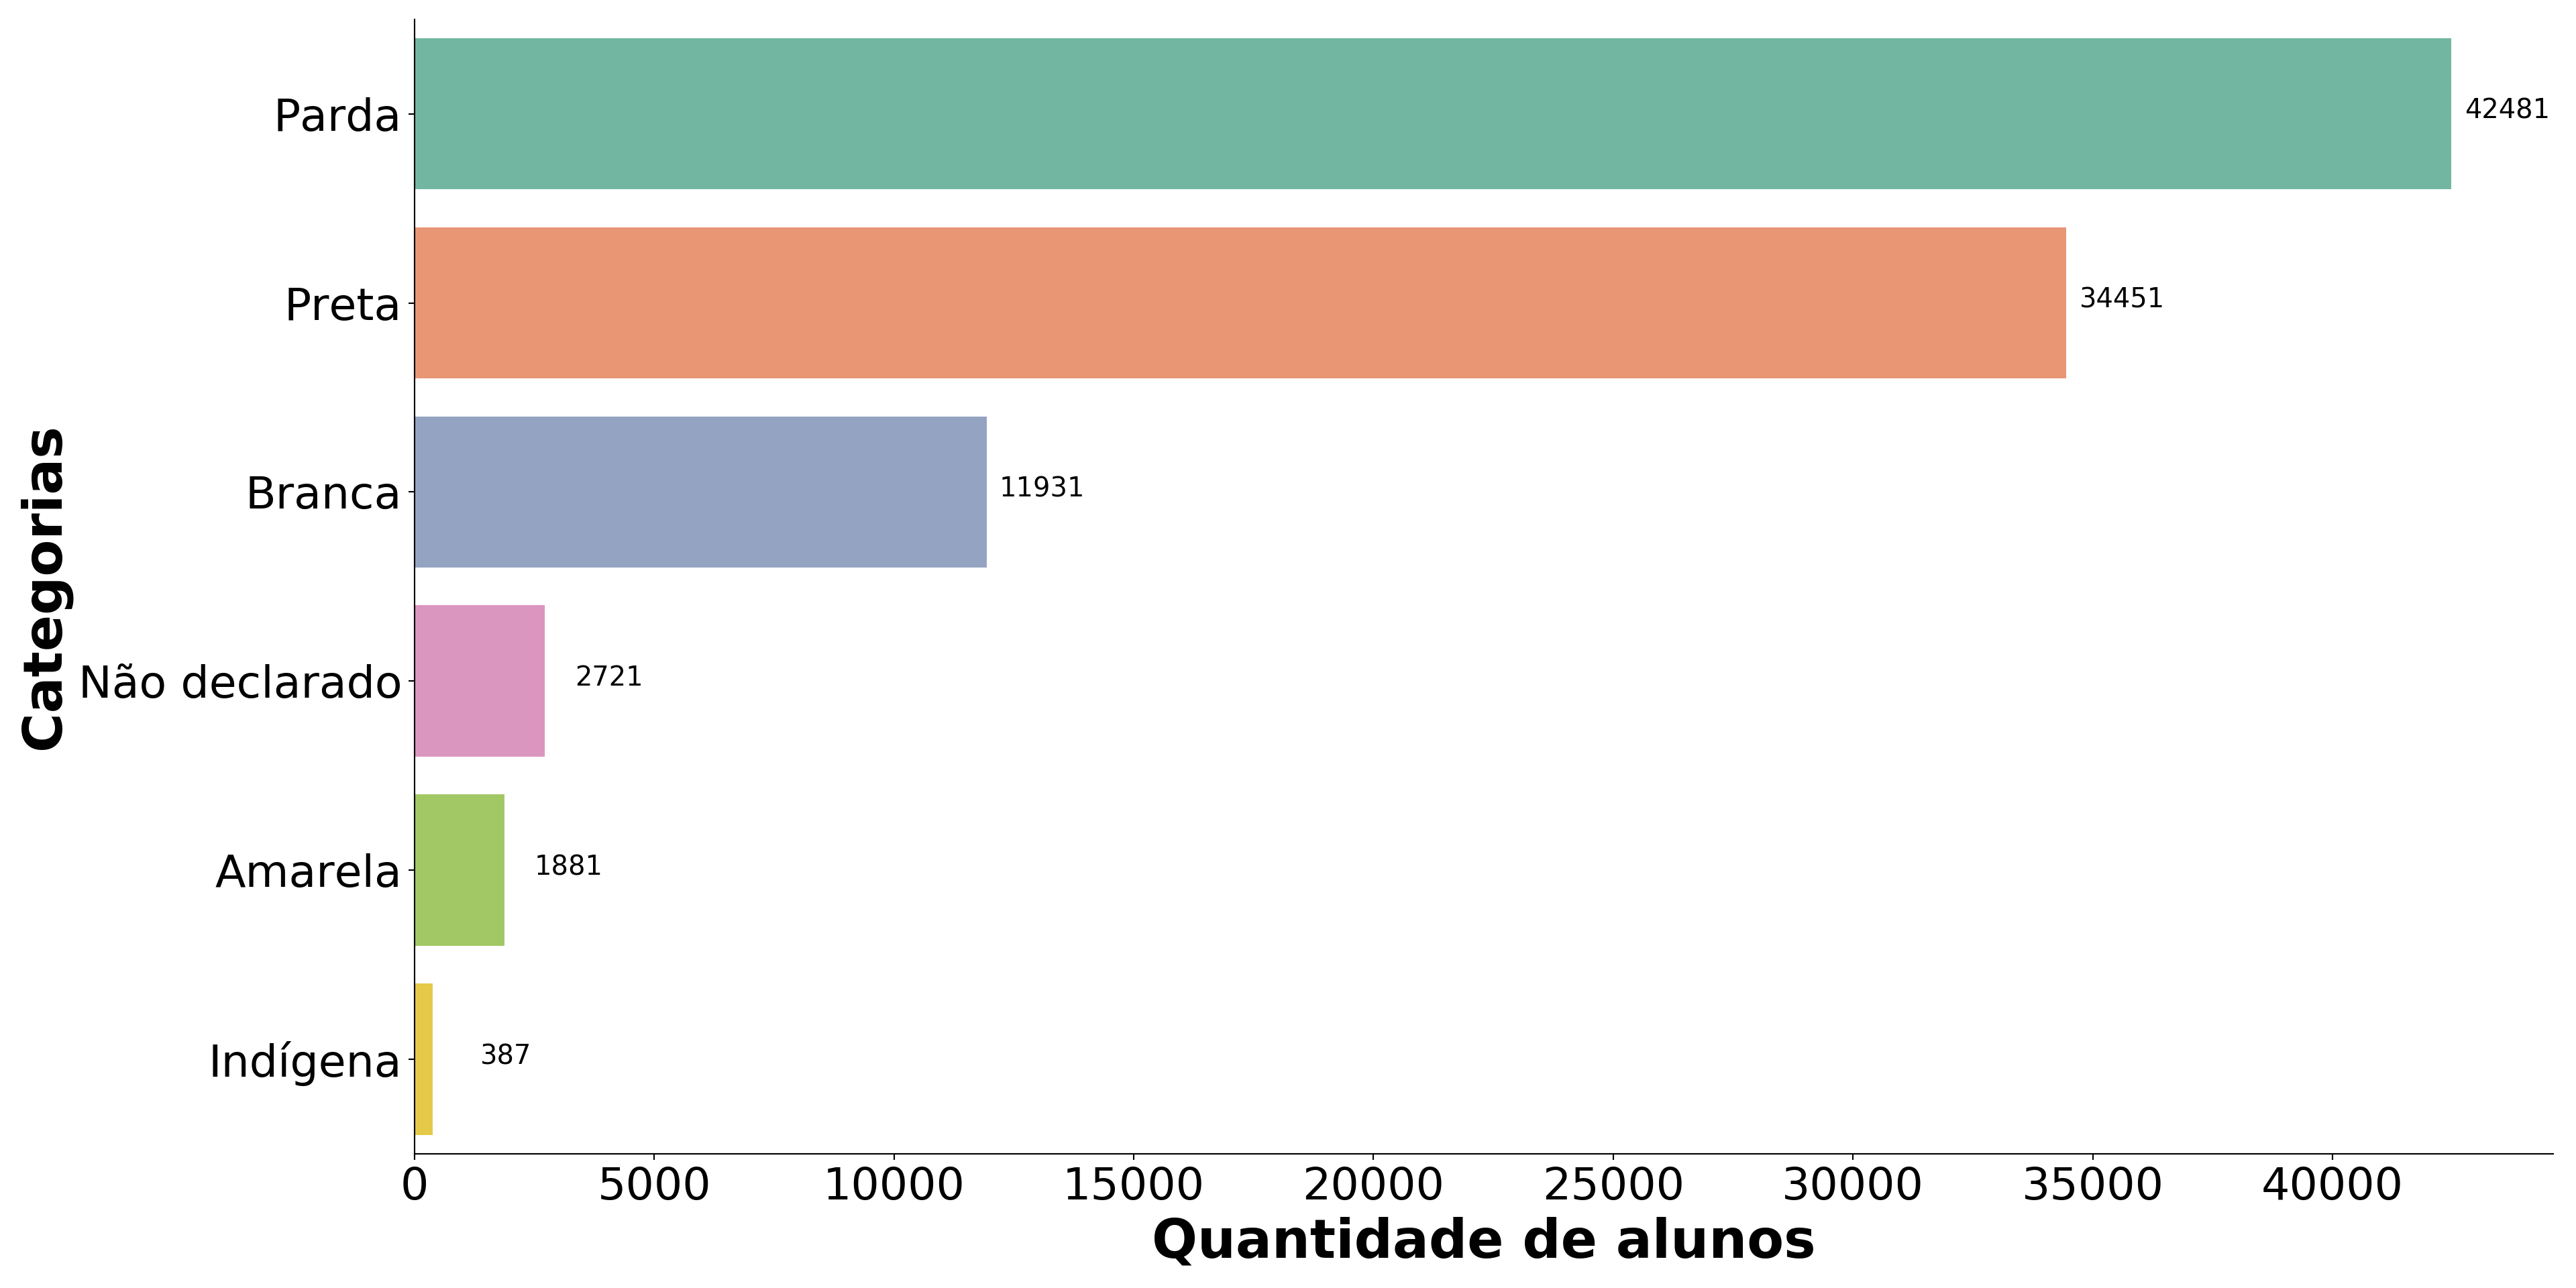
\includegraphics[width=0.9\linewidth]{livro_files/figure-latex/fig32-1} 

}

\caption{Distinção de estudantes por cor/raça da cidade de Salvador inscritos no ENEM 2018 ordenados.}\label{fig:fig32}
\end{figure}

Note como a \texttt{fig32} deixa mais claro outra informação subjetiva: ordem. Com as barras ordenadas, fica mais fácil para o leitor verificar em ordem crescente (do menor para o maior) ou decrescente (do maior para o menor) como está distribuída as categorias naquela variável. Fica mais simples e direto verificar, por exemplo, que a quantidade de estudantes \textbf{Não declarado} é significamente menor que estudantes na categoria \texttt{Pardo} ou \texttt{Preta}.

É importante ressaltar que até o momento foi trabalho apenas com valores absolutos, ou seja, a quantidade total que aquela categoria apareceu naquela variável. Isso é chamado comumente de \textbf{frequência absoluta} (FA). Existe outra forma de dispor esses mesmos valores através da \textbf{frequência relativa} (FR). A frequência relativa é definida como uma proporção dada por:
\[FR = {FA \choose T}\]
Onde \(T\) é o tamanho amostral e \(FA\) a frequência absoluta. Porém é comum apresenta-la no formato \(FR (\%)\) onde ``\%'' indica porcentagem, ou seja, parcela de um todo. Para conseguir essa nova visualização, altera-se a proporção anterior da seguinte forma:
\[FR (\%) = 100*{FA \choose T}\]
A análise utilizando a frequência relativa é bastante usada em pesquisas, pois torna a comparação mais significante. Transformando a \texttt{fig32} de FA para FR obtém-se:

\begin{figure}

{\centering 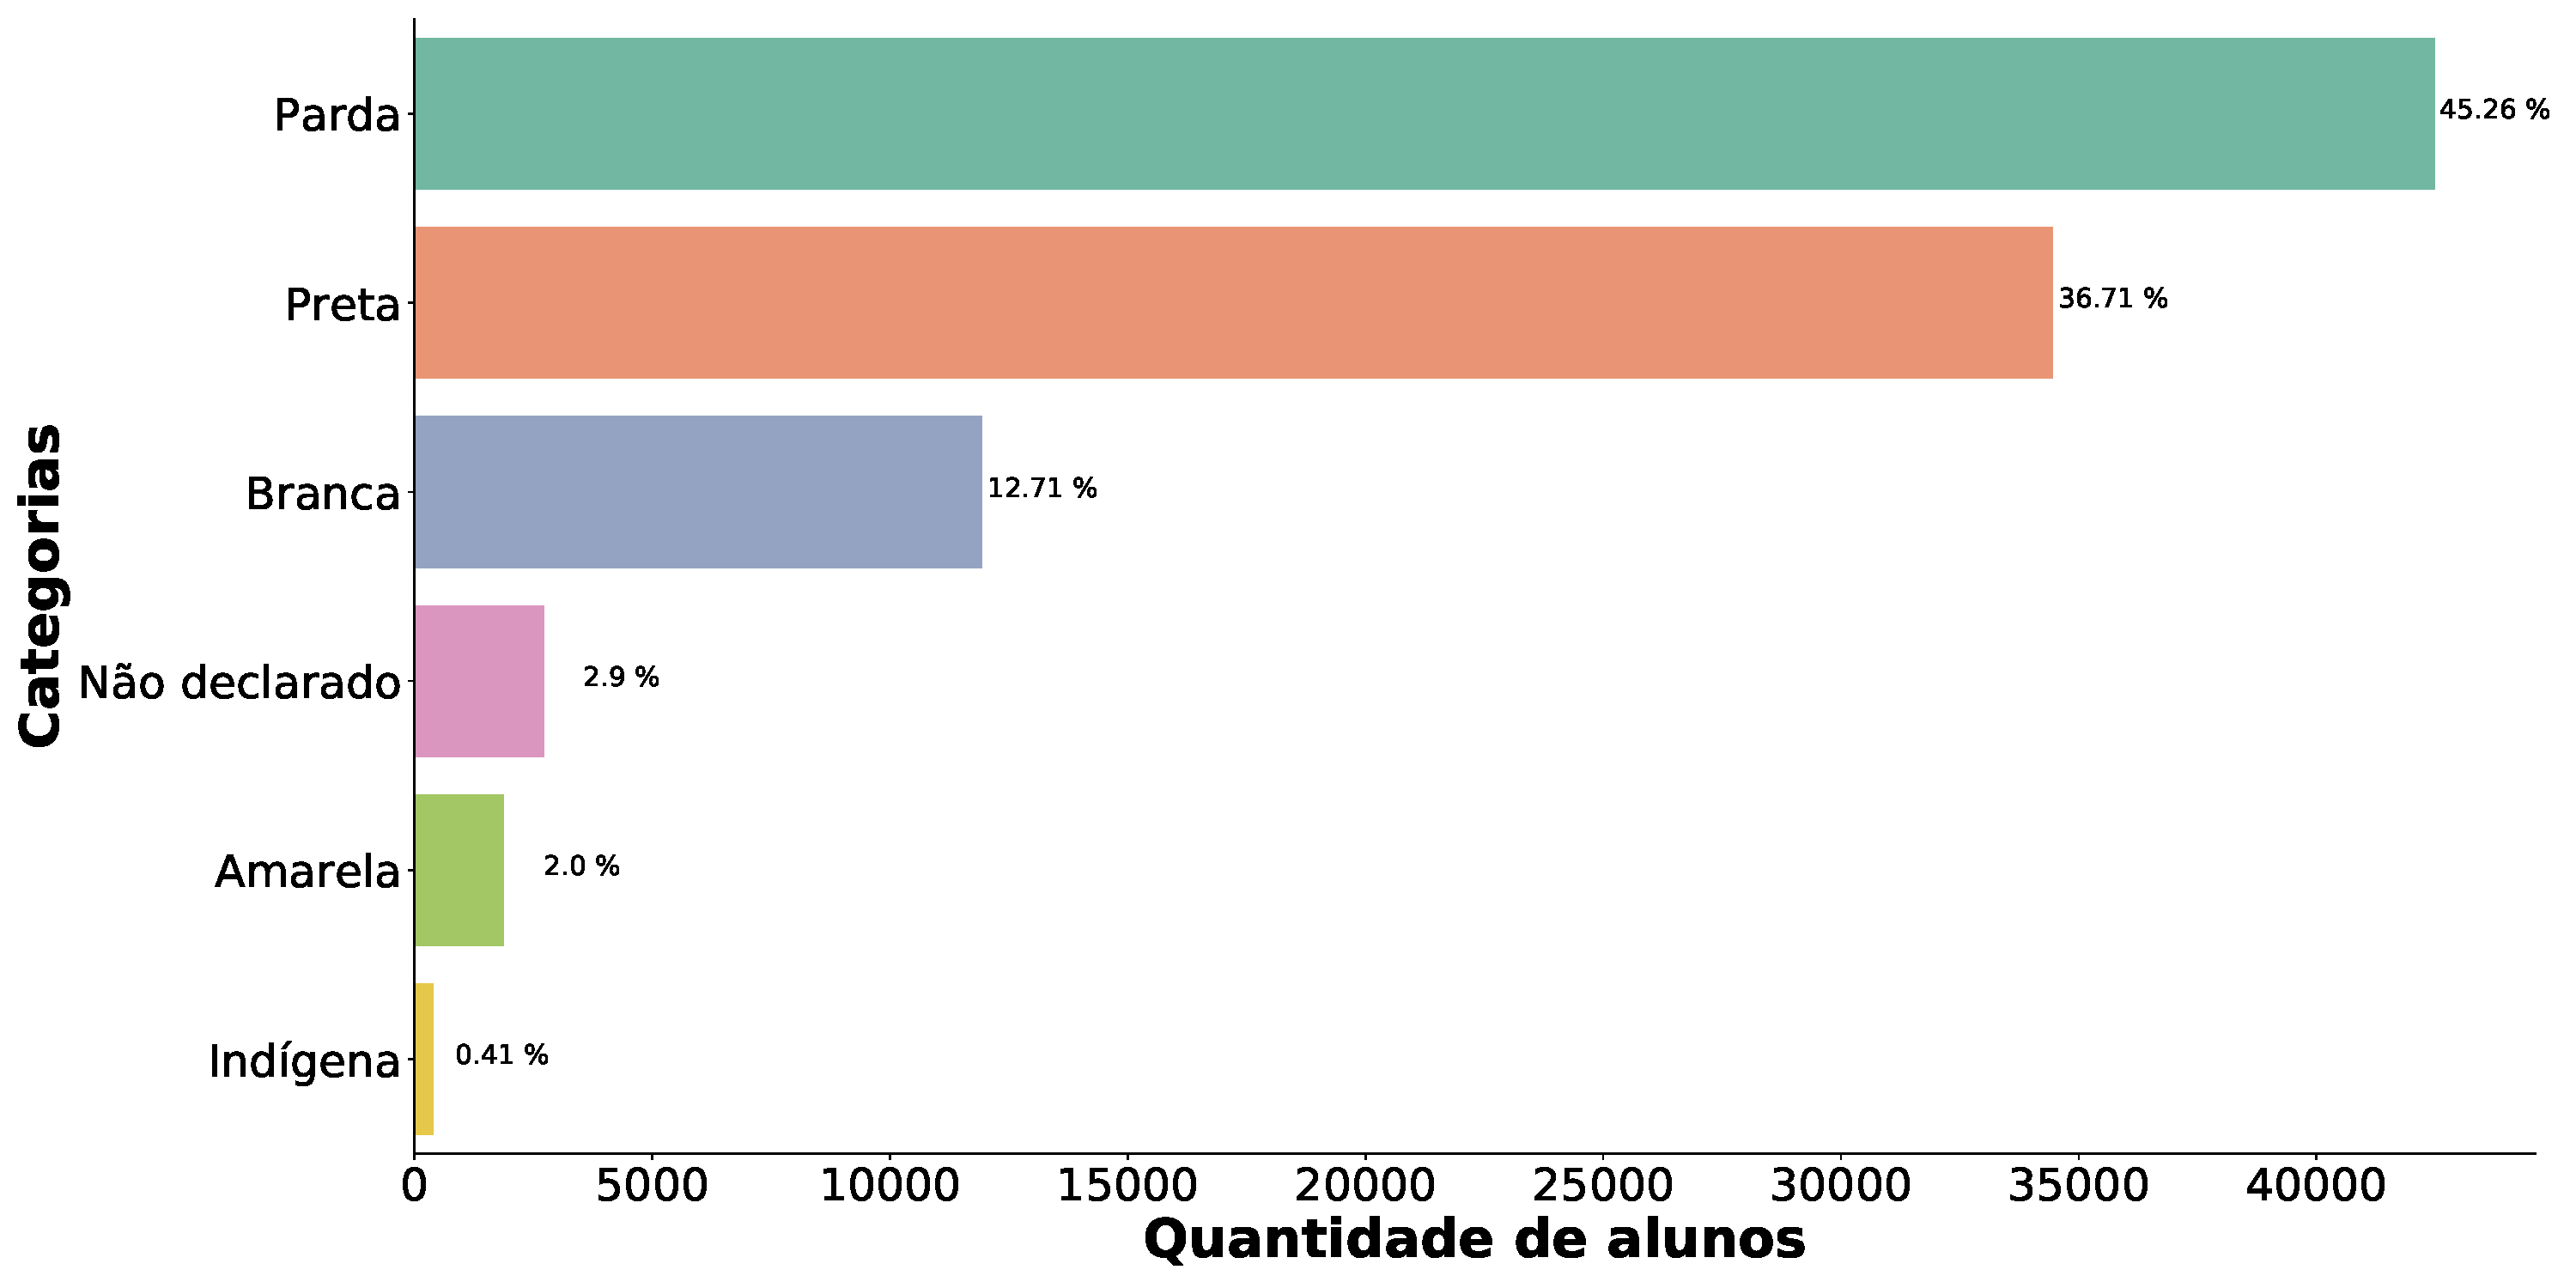
\includegraphics[width=0.9\linewidth]{livro_files/figure-latex/fig33-1} 

}

\caption{Distinção de estudantes por cor/raça da cidade de Salvador inscritos no ENEM 2018 ordenado em frequência relativa.}\label{fig:fig33}
\end{figure}

Ao analisar a \texttt{fig33} você pode perguntar ``Qual é o impacto/diferença em usar FA ou FR?'' ou ``O que eu ganho realizando minha análise com FR?''. Talvez uma análise comparativa entre \texttt{fig32} e \texttt{fig33} possa auxiliar na resolução dessas questões:
- Ao analisar a \texttt{fig33} você identificar que mais de 80\% dos estudantes inscritos no ENEM 2018 são da categoria \texttt{Pardo} ou \texttt{Preta}, verificado ao somar as \(FR(\%)\).
- A quantidade de estudantes ``Não declarado'' é maior do que a quantidade somada de estudantes declarados como \texttt{Indígena} ou \texttt{Amarela}.

Essa informações expressivas de quantidades não poderiam ser verificadas na \texttt{fig32} visto que não fica claro o tamanho amostral na \(FA\), apenas na \(FR(\%)\).Toda essa análise mostra como um gráfico pode ser aperfeiçoado com o tempo e como um gráfico de barras pode conter tantas informações. Vale ressaltar que inclusive essa predominância de pessoas auto declaradas de cor \texttt{Parda} ou \texttt{Preta} reflete a realidade da capital mais negra do Brasil segundo o censo de 2018 do Instituto Brasileiro de Geografia e Estatística (IBGE).

Apesar do gráfico de barras estar bastante relacionado com variáveis categóricas, ele pode ser usado também para expressar grandezas numéricas de uma forma visual. Isso é realizado na imagem seguinte:

\begin{figure}

{\centering 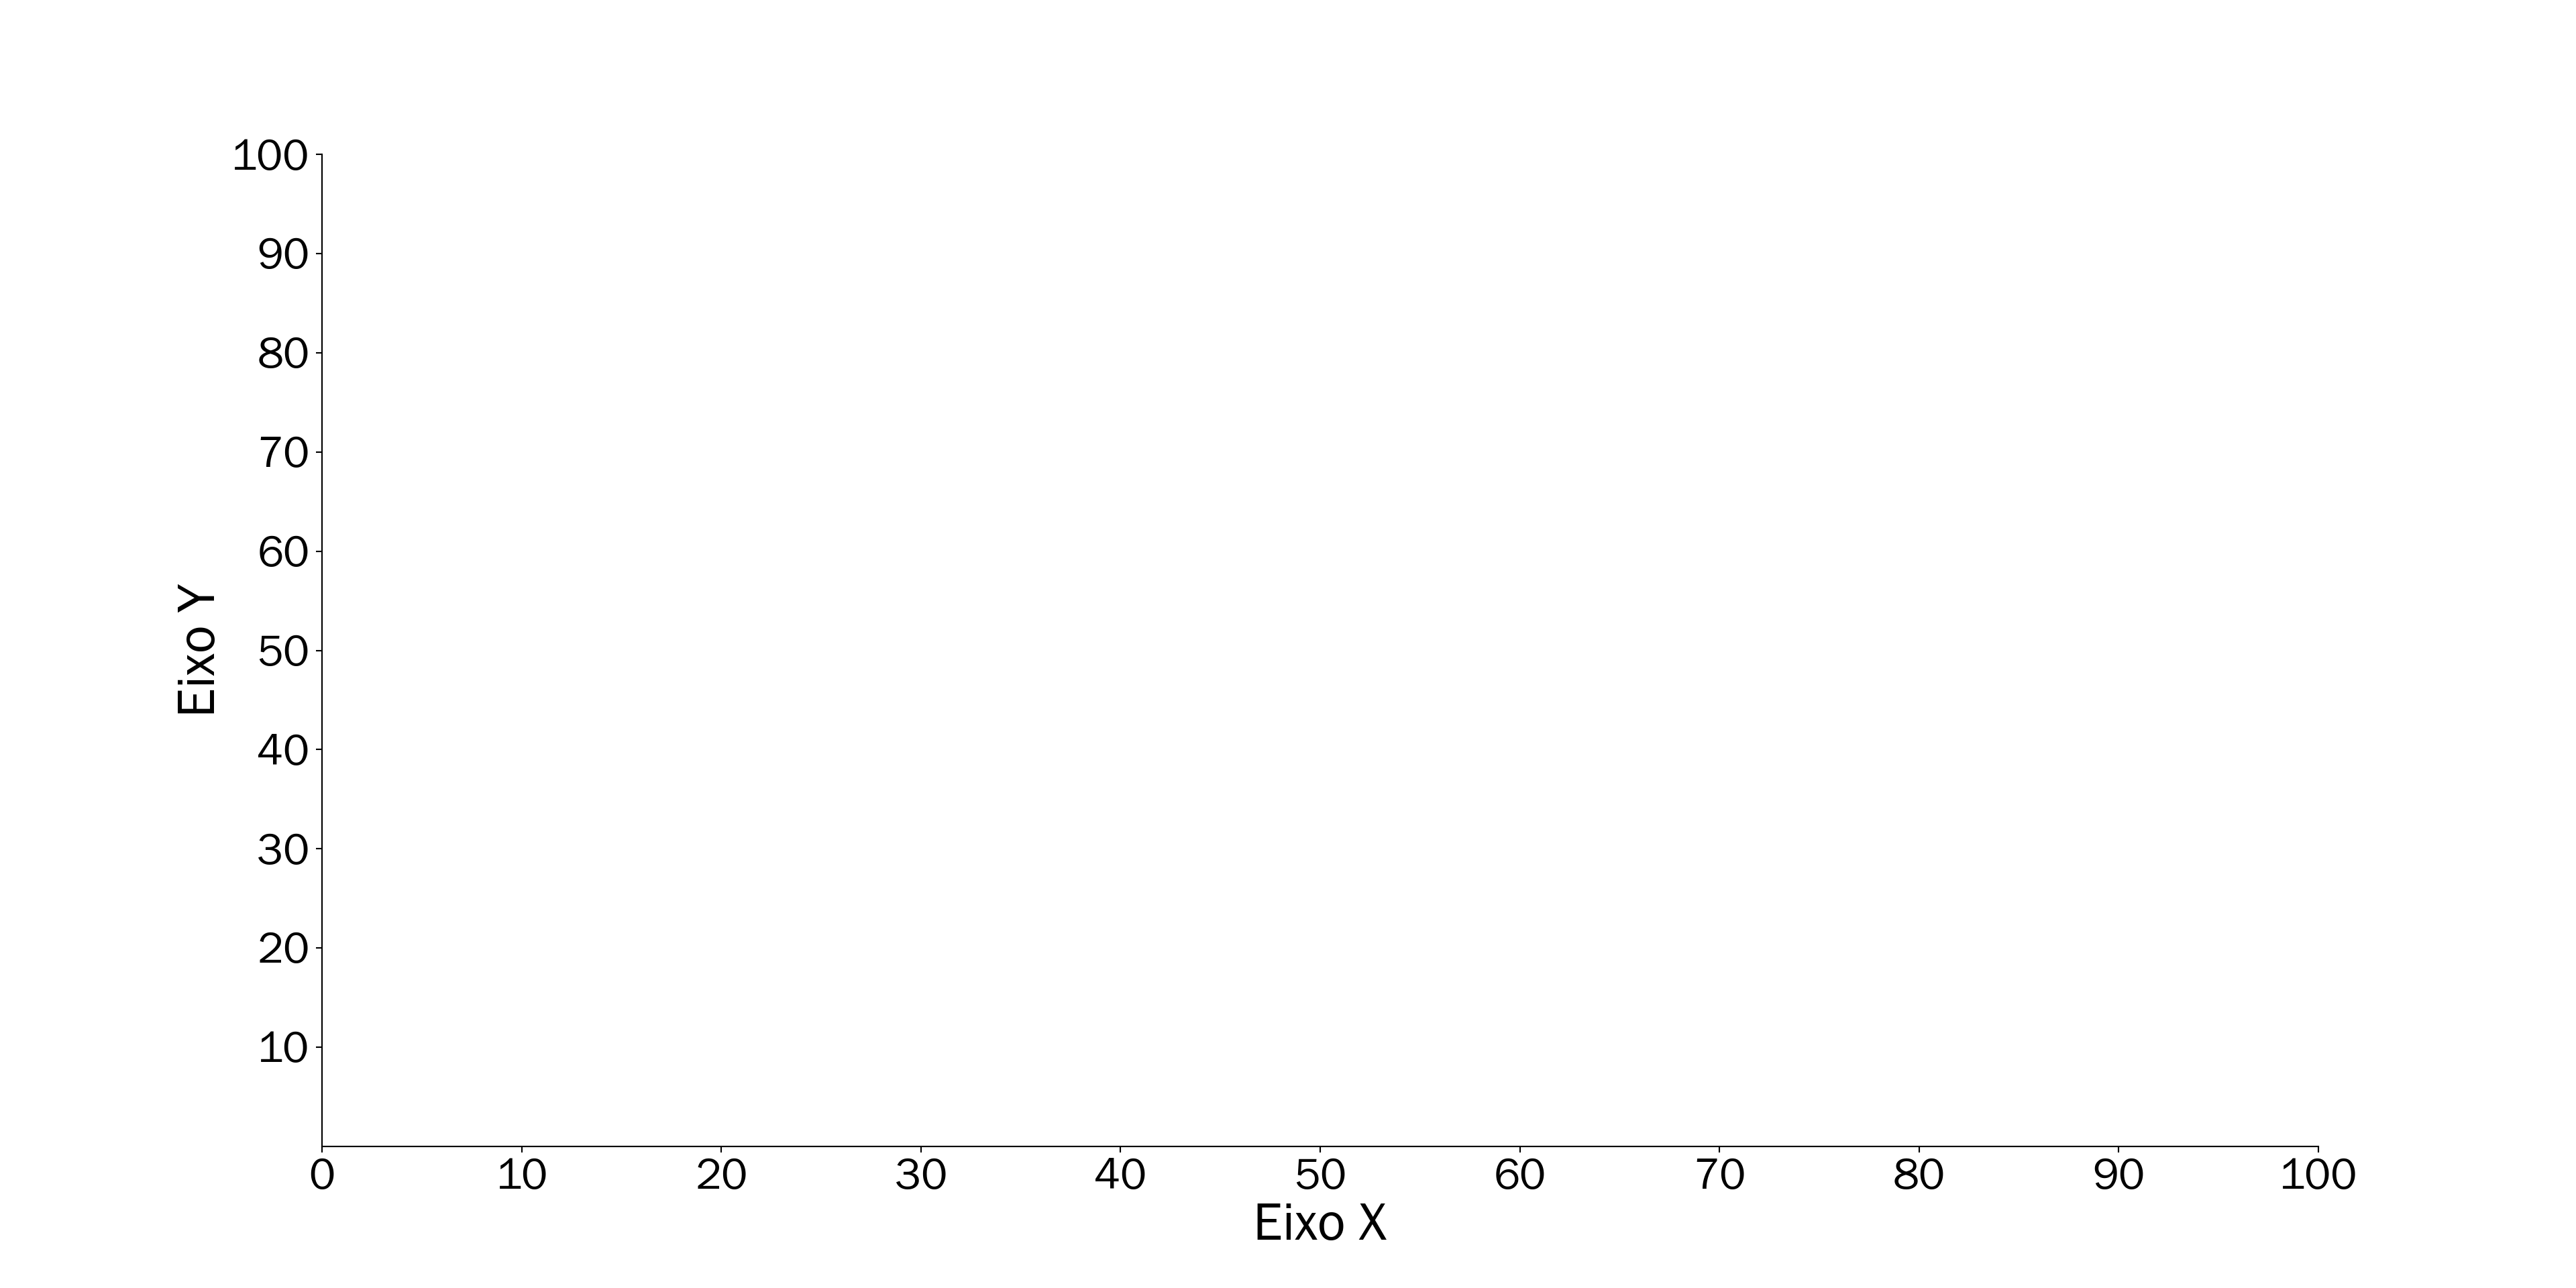
\includegraphics[width=0.9\linewidth]{livro_files/figure-latex/fig34-1} 

}

\caption{Notas máximas e mínimas no ENEM 2018 para os estudantes de Salvador (BA).}\label{fig:fig34}
\end{figure}

A \texttt{fig34} apesar de não apresentar variáveis com nenhum teor categórico, pois as notas de provas apresentam um caráter numérico, demonstra a utilização do gráfico de barras para demonstrar a discrepância entre as maiores e menores notas para as diversas provas do ENEM (desconsiderando provas zeradas). A utilização deste tipo de gráfico com esse viés é interessante para ressaltar diferenças principalmente em resultados, fazendo com que o leitor perceba como um valor é superior ou inferior que o outro.

\hypertarget{gruxe1fico-de-pizza}{%
\section{Gráfico de pizza}\label{gruxe1fico-de-pizza}}

O \textbf{Gráfico de pizza}, também conhecido como gráfico de setores, pode ser visto como uma forma alternativa ao \textbf{gráfico de barras} para expressar informações . Neste gráfico, construído exclusivamente para variáveis categóricas, cada fatia referente a uma categoria possui um tamanho proporcional a \(FR(\%)\) . Abaixo é apresentado um exemplo desta modalidade:

\begin{figure}

{\centering 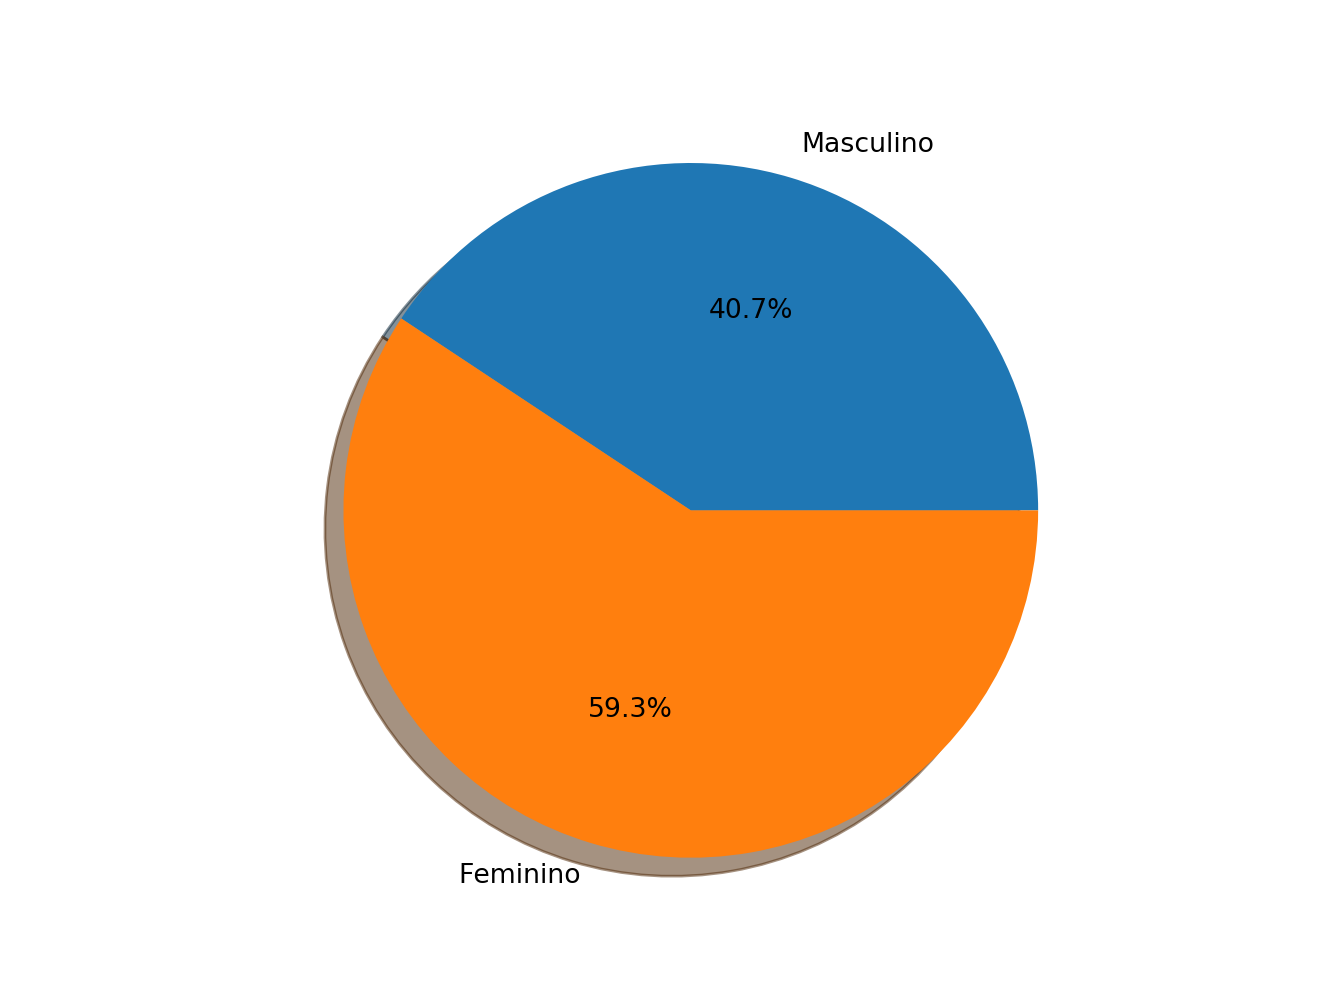
\includegraphics[width=0.9\linewidth]{livro_files/figure-latex/fig35-1} 

}

\caption{Quantidade de alunos do sexo masculino e feminino inscritos no ENEM 2018.}\label{fig:fig35}
\end{figure}

Através da análise da \texttt{fig35} é possível identificar que a proporção de estudantes do sexo feminino é maior do que do sexo masculino. Isso é verificado pelo tamanho da \(FR(\%)\) e também pela ``fatia'' dessa categoria. Neste tipo de gráfico, a categoria mais dominante irá apresentar um tamanho maior em comparação as demais, caso isso não ocorra provavelmente existe alguma coisa errada com seu gráfico.

A análise utilizando um gráfico de pizza é interessante quando é estudado uma variável categórica em específico e almeja apresentar possíveis dominâncias entre suas classes. Essa abordagem, todavia, não é recomendado quando o atributo estudado apresenta muitas categorias, pois a visualização se torna mais difícil para o leitor. Neste caso é recomendado a utilização dos gráficos de barras.

\hypertarget{gruxe1ficos-de-dispersuxe3o}{%
\section{Gráficos de Dispersão}\label{gruxe1ficos-de-dispersuxe3o}}

\hypertarget{suxe9ries-temporais}{%
\section{Séries temporais}\label{suxe9ries-temporais}}

A \textbf{série temporal}, comumente chamada de gráfico de linha, se trata de uma coleção de observações realizadas ao longo do tempo. Por se tratar de uma coleta sequencial, ou seja, feita uma após a outra torna o fator de ordenação fundamental: importa saber se determinada observação ocorreu antes ou depois de determinado evento. Um exemplo muito conhecido deste tipo de gráfico, presente no dia a dia do leitor é a previsão do tempo em jornais: lhe é apresentado as previsões para o dia presente e alguns dias futuros da semana. Outro exemplo dessa análise é apresentado abaixo:

\begin{figure}

{\centering 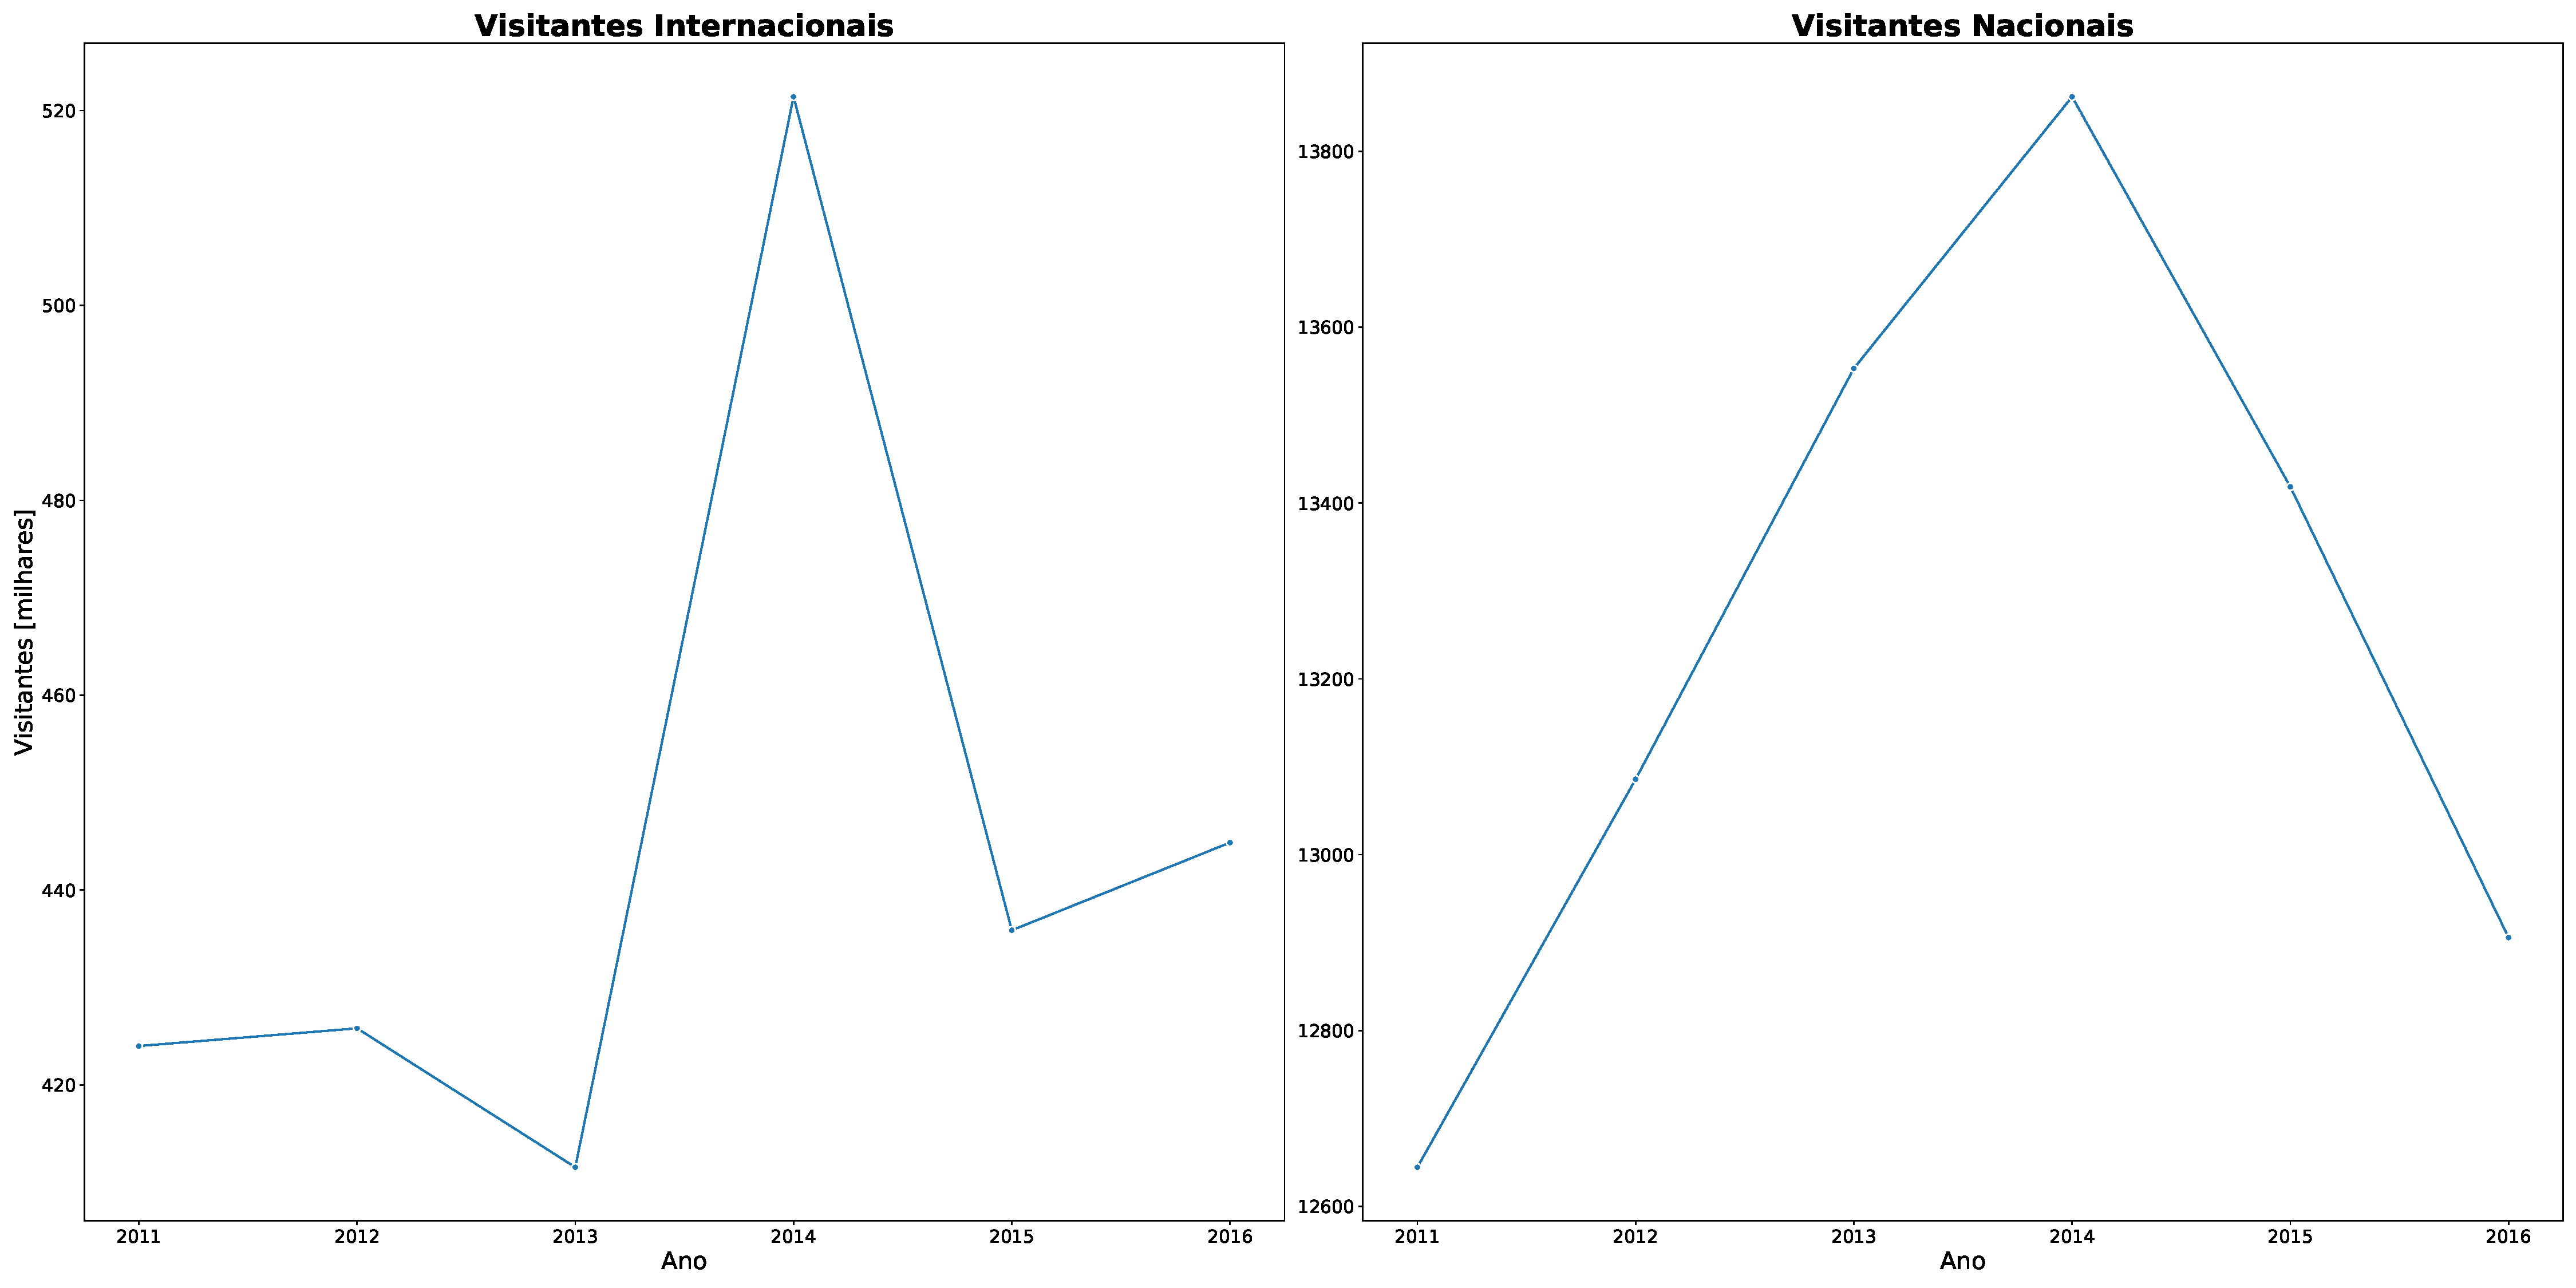
\includegraphics[width=0.9\linewidth]{livro_files/figure-latex/fig36-1} 

}

\caption{Fluxo turístico na capital da Bahia nos anos de 2011 até 2016.}\label{fig:fig36}
\end{figure}

As séries temporais apresentadas na \texttt{fig36} apresentam o fluxo turístico internacional (a esquerda) e nacional (a direita) em Salvador. É possível avaliar através destes gráficos que 2014 apresentou um enorme fluxo tanto nacional quanto internacional em Salvador. Este aumento expressivo identificado em um determinado período em comparação com os demais é chamada de \textbf{pico}. A ocorrência de um pico é comumente atrelada a um evento inesperado que pode explicar sua origem. Neste caso em específico, o aumento expressivo de turistas em Salvador pode ser relacionado a Copa do Mundo de 2014, maior evento de futebol do mundo, sediada no Brasil onde alguns jogos aconteceram na capital bahiana. Esse fato é corroborado pela raridade dessa ocorrência (primeira vez que ocorreu) e pela diferença deste período em comparação aos anos anteriores e posteriores a 2014.

Além de avaliar eventos únicos que possam ter ocorrido, buscando compreendê-los, as séries temporais são ferramentas essenciais para acompanhar um determinado processo ou fluxo, podendo auxiliar na tomada de decisões.

\begin{figure}

{\centering 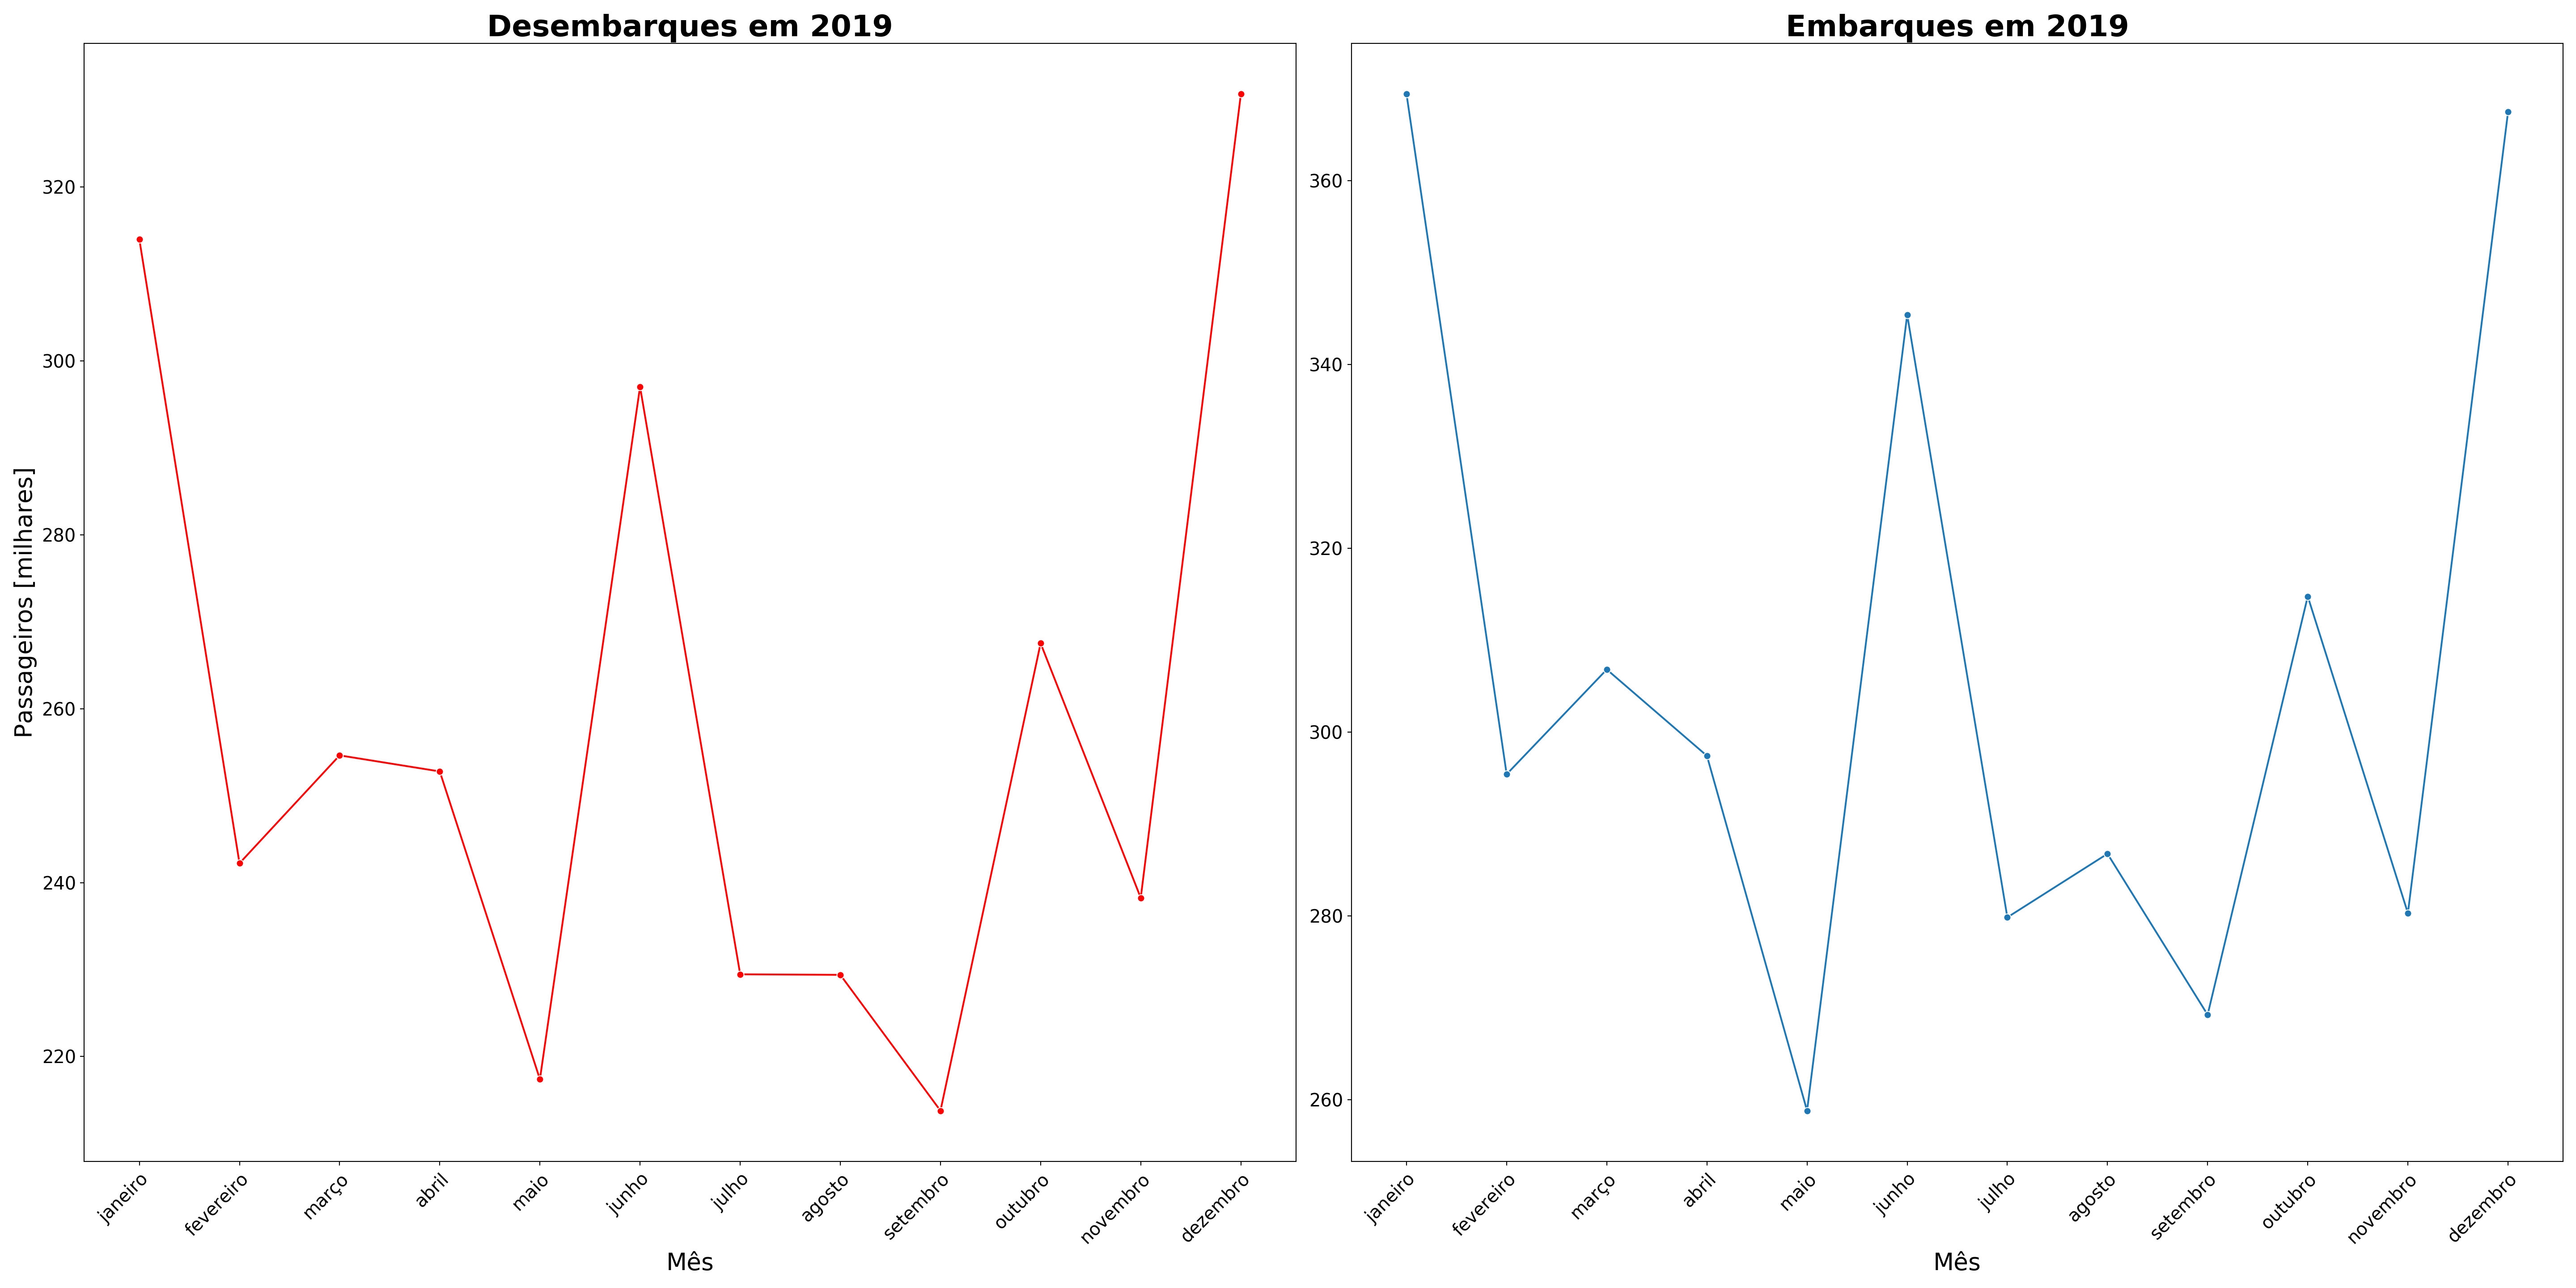
\includegraphics[width=0.9\linewidth]{livro_files/figure-latex/fig37-1} 

}

\caption{Fluxo de desembarques e embarques no terminal rodoviário de Salvador em 2019.}\label{fig:fig37}
\end{figure}

As informações contidas na Figura \texttt{fig37} podem ser interessantes, por exemplo, para um gestor público responsável pelo terminal rodoviário de Salvador que pode identificar:
- durantes os meses de Janeiro, Junho e Dezembro ocorrem os períodos de maiores movimentações tanto para embarque quanto para desembarque. Isso pode indicar a necessidade de mais investimentos/atenção dos funcionários do terminal para garantir a movimentação sem grandes transtornos.
- os meses de Maio e Setembro apresentam o menor movimento. Logo, o investimento neste período pode ser reduzido em detrimento de meses com maiores movimentações como Janeiro e Dezembro.

Ou seja, a compreensão de gráficos deste tipo podem ajudar na tomada de decisões durante o gerenciamento através da compreensão de períodos importantes.

\hypertarget{histograma}{%
\section{Histograma}\label{histograma}}

Um histograma de um conjunto de dados numéricos se parece muito com um gráfico de barras apresentado anteriormente, embora tenha algumas diferenças importantes que examinaremos nesta seção. Primeiro, abaixo é apresentado um histograma para mostrar a distribuição da idade dos participantes do ENEM 2018 na cidade de Salvador:

\begin{figure}

{\centering 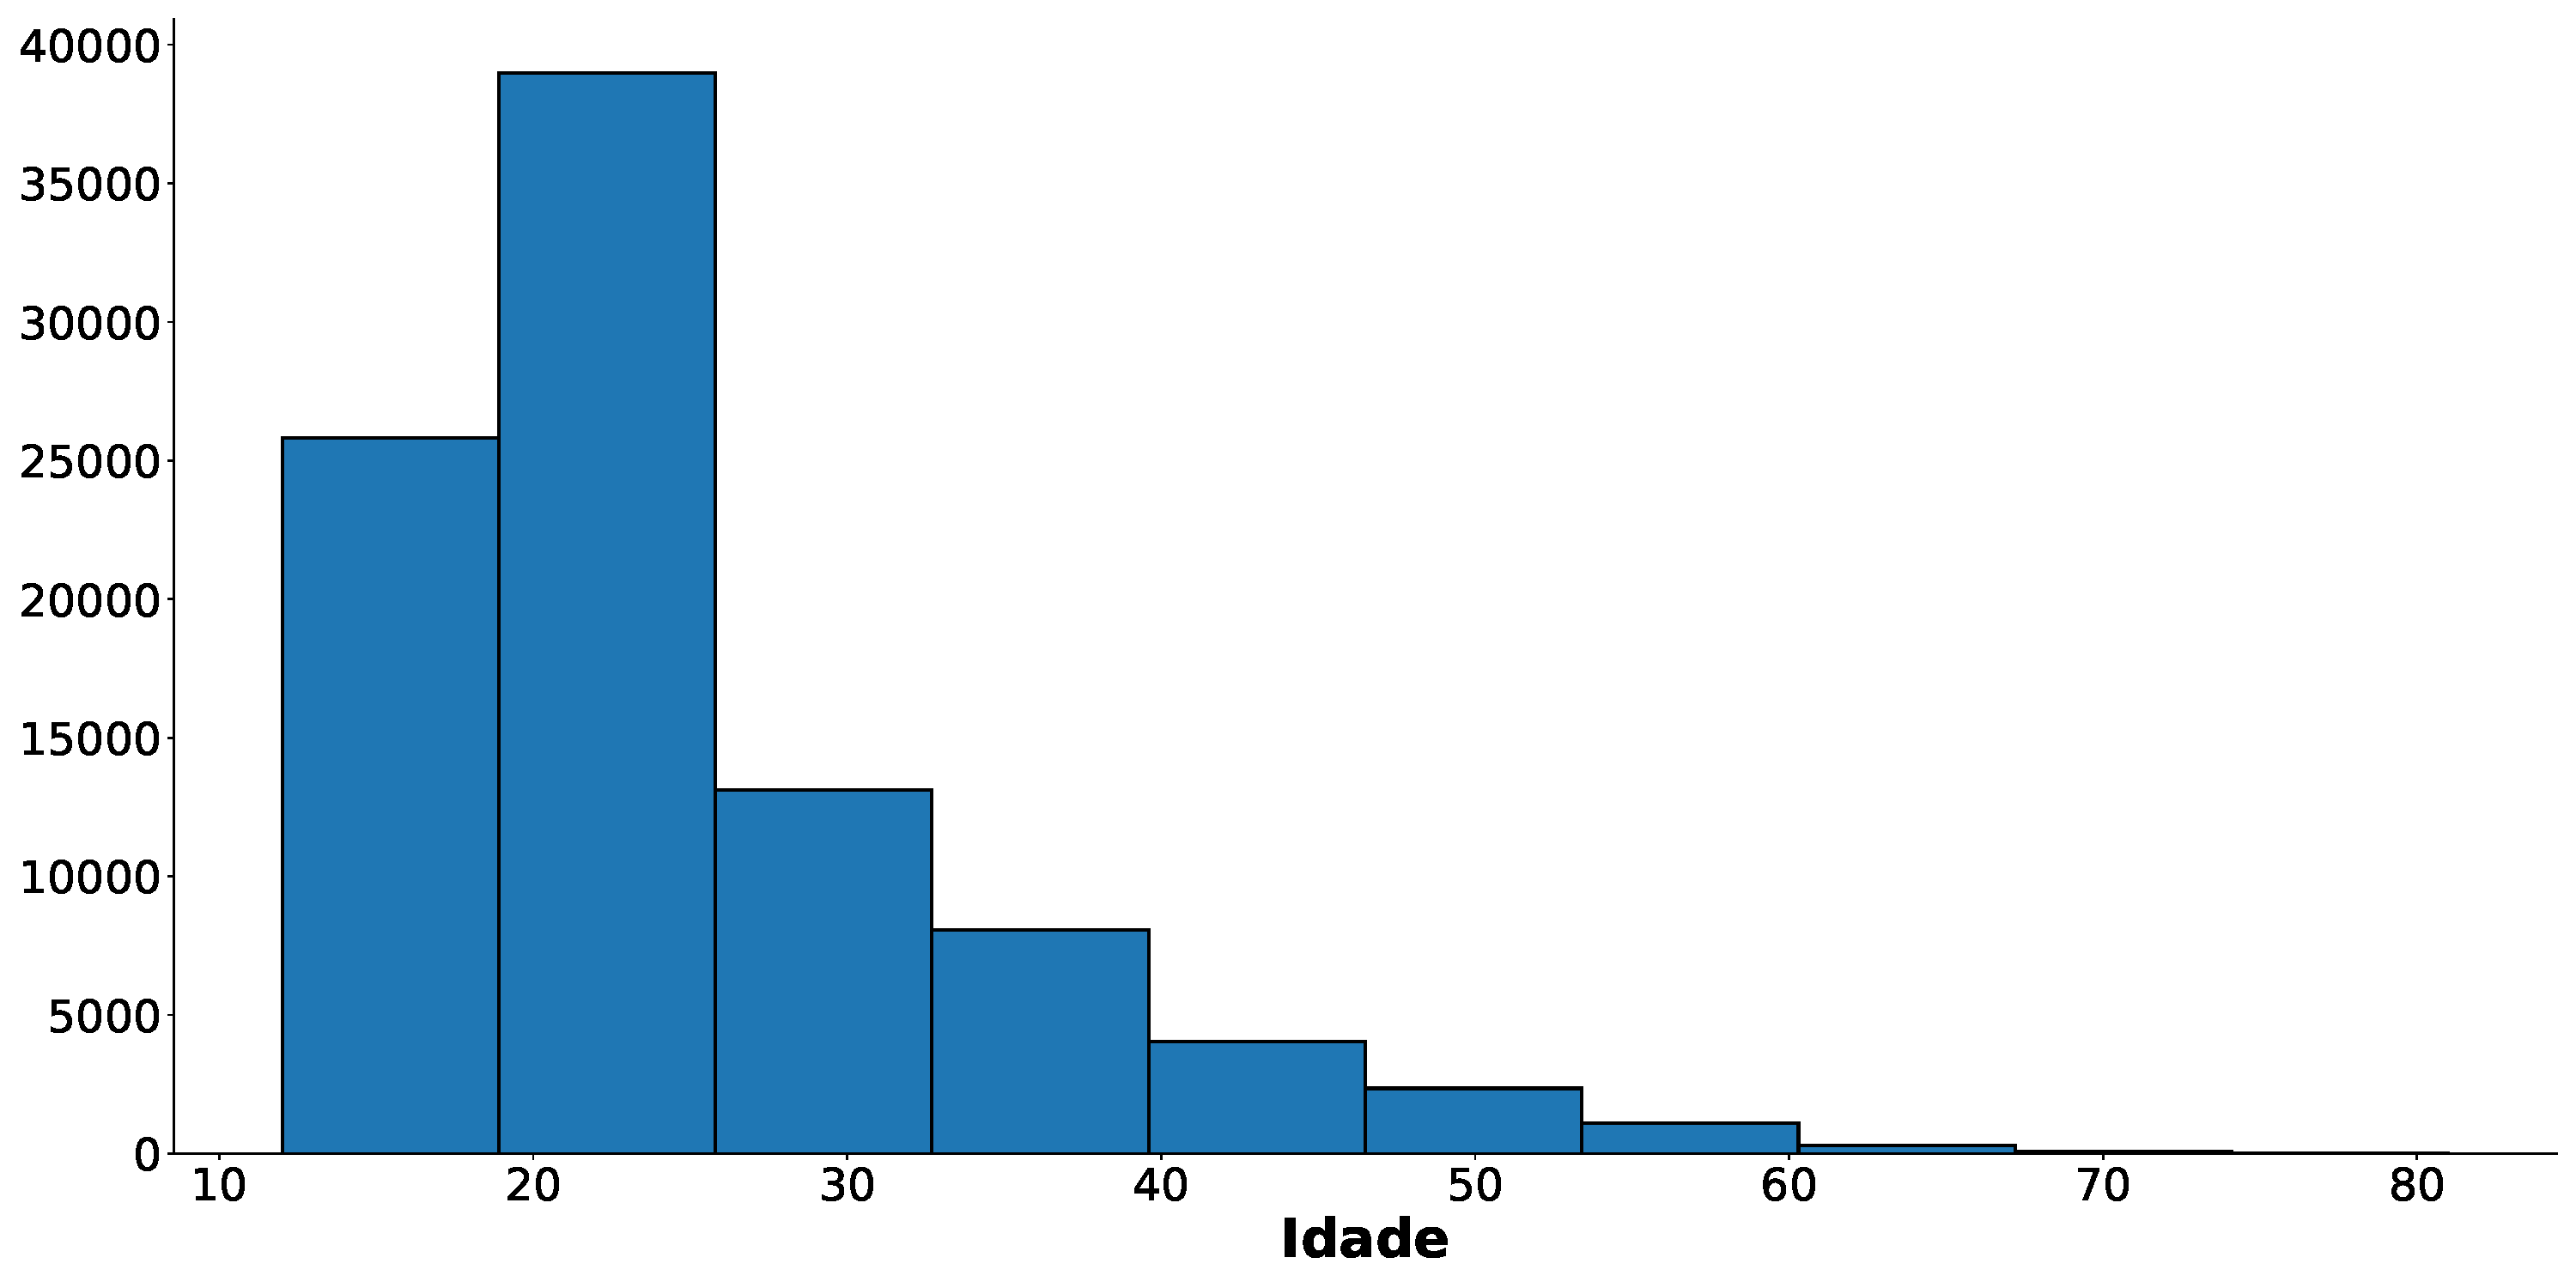
\includegraphics[width=0.9\linewidth]{livro_files/figure-latex/fig38-1} 

}

\caption{Histograma da idade dos participantes do ENEM 2018 na cidade de Salvador}\label{fig:fig38}
\end{figure}

No eixo horizontal está representado os valores numéricos da idade dos participantes do ENEM que foram agrupados em intervalos discretos. Fazendo um paralelo com o \ref{capitulo-2}, o intervalo contínuo numérico estudado foi transformado para \textbf{K} valores categóricos/discretos. Este valor \textbf{K} é definido pelo usuário e na imagem anterior é definido como igual a 10. Você pode perceber isso ao contar a quantidade de ``caixinhas'' que existem no histograma. Já o eixo vertical representa a quantidade de valores que estão em cada categoria, ou seja, quanto mais valores são representados por aquela classe maior será a altura de sua barra. Caso você esteja afiado, provavelmente notou uma semelhança com a frequência absoluta apresentada durante a seção @ref(\#graficos-de-barras).

Ao avaliar um histograma é preciso entender que cada barra representa uma categoria que define um intervalo contínuo limitado. Esse intervalo é na maioria das vezes apresentado da seguinte forma:
\[[limite\ inferior,\ limite\ superior)\]
Onde o \(limite\ inferior\) representa o menor valor contido naquela categoria e \(limite\ superior\) o maior valor daquela categoria. Porém, na matemática os sinais \([\) e \()\) apresentam um significado específico, importantes para compreender a definição de uma categoria do histograma: o primeiro representa um intervalo fechado já o segundo um intervalo aberto. Juntando todo este conhecimento é possível dizer que cada K categoria em um histograma contém seu limite inferior, mas não contém seu limite superior. Em outras palavras, uma determinada barra (categoria) não representa seu limite superior, logo uma categoria começa no limite inferior e termina no superior, sem inclui-lo.

Na \texttt{fig38} é possível observar que com 10 categorias, a medida que aumenta a idade dos participantes mais difícil se torna difícil enxergar as barras. Além disso, a categoria mais dominante se encontra na faixa dos 18 aos 26 anos. Caso seja desejado aumentar a resolução desses intervalos, será necessário realizar o aumento de categorias e isso pode ser conquistado ao aumentar o valor de K.

\begin{figure}

{\centering 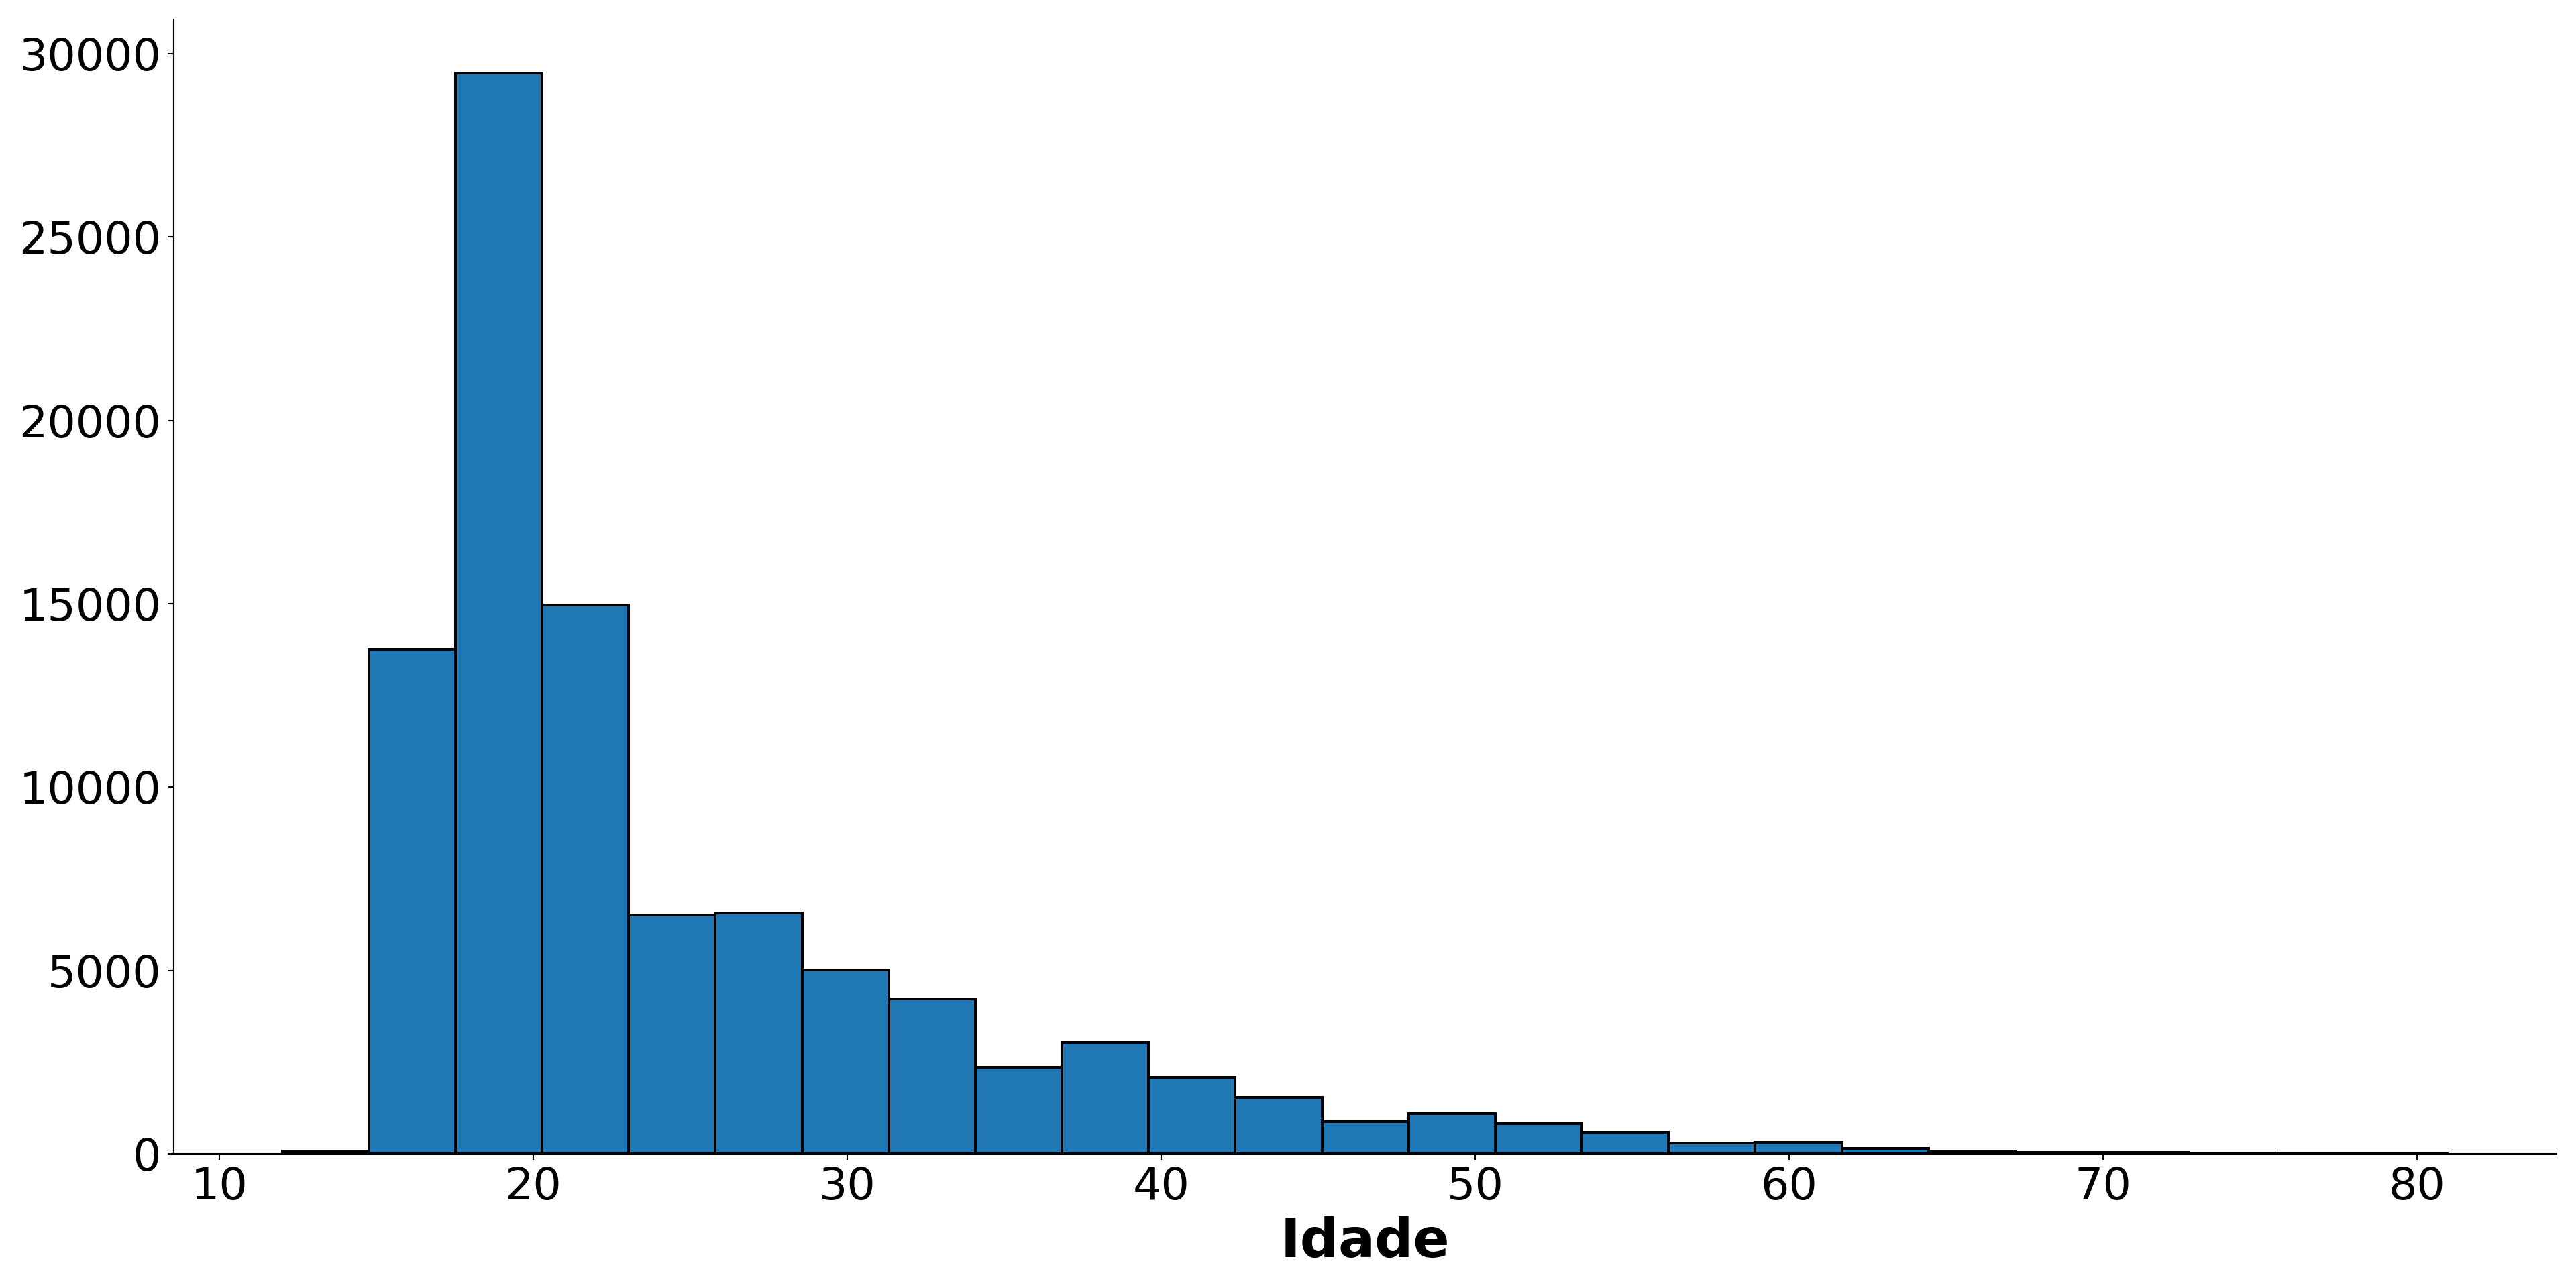
\includegraphics[width=0.9\linewidth]{livro_files/figure-latex/fig39-1} 

}

\caption{Histograma da idade dos participantes do ENEM 2018 na cidade de Salvador com uma maior resolução}\label{fig:fig39}
\end{figure}

Ao utilizar 25 categorias, como apresentado na \texttt{fig39} é possível identificar que o intervalo de idade mais dominante foi anulado para participantes com idade em torno de 15 aos 21 anos, o que é congruente visto que a maioria dos inscritos no ENEM são estudantes do ensino médio. Essa conclusão é corroborada com a queda da no eixo vertical para idades superiores a 20 anos.

Para corroborar ainda mais essa ideia vamos analisar o gráfico abaixo:

\begin{verbatim}
## ([<matplotlib.patches.Wedge object at 0x0000000043E3D0C8>, <matplotlib.patches.Wedge object at 0x0000000043E3D988>], [Text(0.13351534689450067, 1.091867048748904, 'Abaixo dos 20 anos'), Text(-0.13351524466652911, -1.091867061249508, 'Acima dos 20 anos')], [Text(0.07282655285154582, 0.5955638447721293, '46.1%'), Text(-0.07282649709083405, -0.5955638515906407, '53.9%')])
\end{verbatim}

\begin{verbatim}
## (-1.1096569746405915, 1.1004598837057975, -1.111390396575388, 1.1238395526998675)
\end{verbatim}

\begin{figure}

{\centering 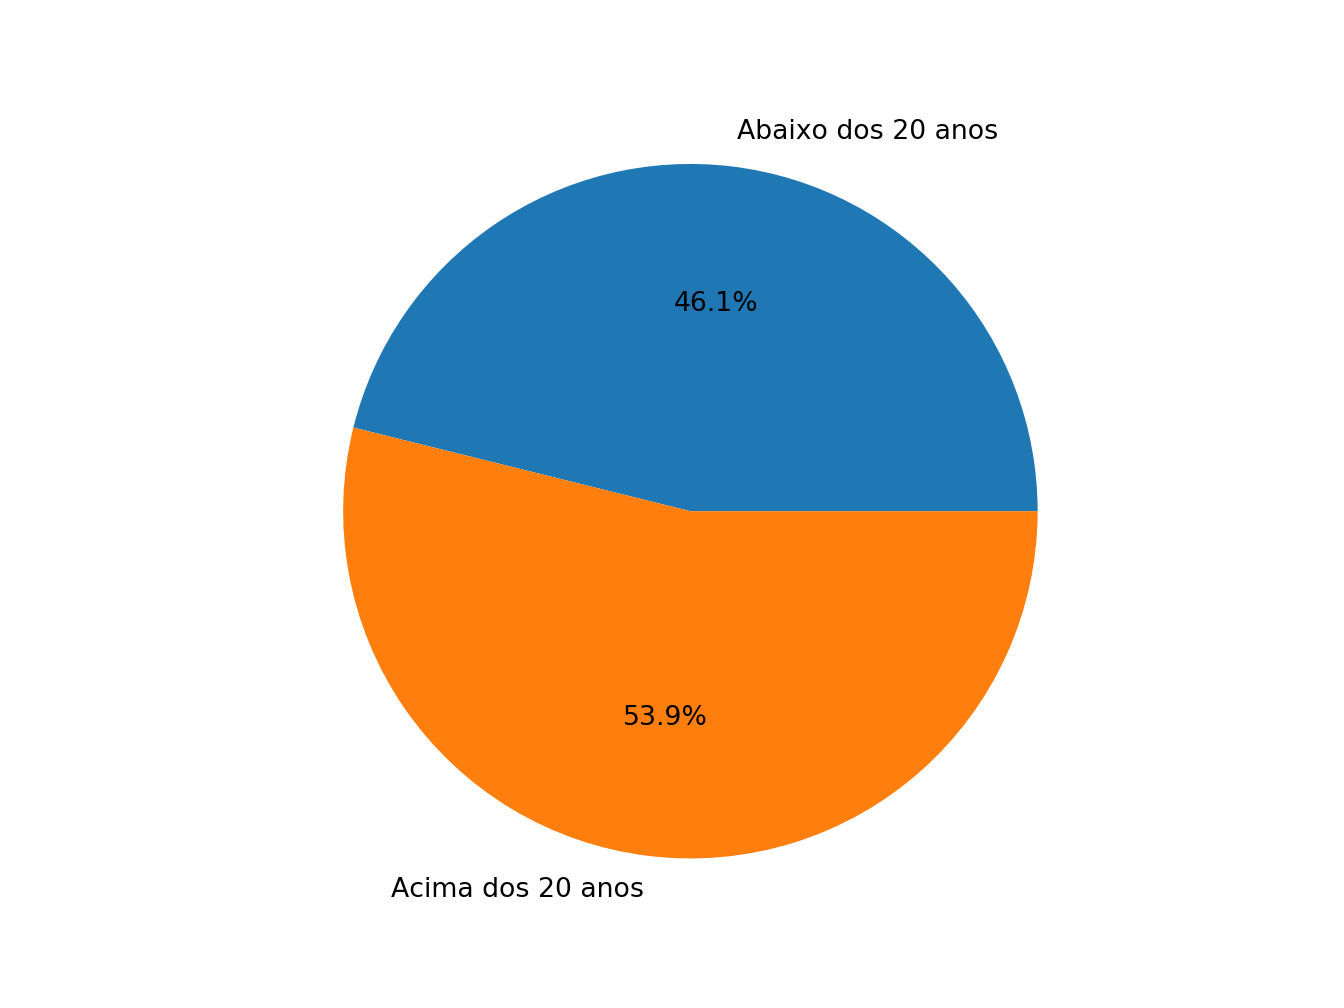
\includegraphics[width=0.9\linewidth]{livro_files/figure-latex/fig310-1} 

}

\caption{Histograma da idade dos participantes do ENEM 2018 na cidade de Salvador com uma maior resolução}\label{fig:fig310}
\end{figure}

O gráfico de pizza exposto na \texttt{fig310} avalia a quantidade de estudantes de acordo ao um limite de 20 anos de idade. É verificado que quase 50\% dos participantes do ENEM 2018 apresentam uma idade inferior a 20 anos, solidificando ainda o que foi verificado durante a a análise do histograma passado, mesmo com um intervalo de idade que vai desde os 12 anos até 81 anos verificado.

Após concluir a leitura desta seção você pode notar a semelhança entre \textbf{histograma} e \textbf{gráfico de barras}, porém não confunda: eles são diferentes! Suas principais diferenças são:
- Os gráficos de barras exibem uma quantidade por categoria. Eles são frequentemente usados para exibir as distribuições de variáveis categóricas. Os histogramas exibem as distribuições de variáveis numéricas.
- Todas as barras em um gráfico de barras têm a mesma largura e há uma quantidade igual de espaço entre as barras consecutivas. As barras de um histograma podem ter larguras diferentes e são contíguas.

\textbf{Nota}: É importante ressaltar que alguns materiais trazem o conceito da densidade para o eixo vertical, porém dado o direcionamento do livro será mantido uma análise sem abordar este conceito dado a sua complexidade. A ideia de densidade é importante quando é analisado histogramas com intervalos de tamanhos diferentes, mas para intervalos iguais tanto o conceito de frequência absoluta (contagem) quanto densidade funcionam para o mesmo propósito.

\hypertarget{aprimorando-suas-visualizauxe7uxf5es}{%
\section{Aprimorando suas visualizações}\label{aprimorando-suas-visualizauxe7uxf5es}}

\hypertarget{indo-aluxe9m}{%
\section{Indo Além \ldots{}}\label{indo-aluxe9m}}

\hypertarget{referuxeancias}{%
\section{Referências}\label{referuxeancias}}

\url{https://pt.wikipedia.org/wiki/Gr\%C3\%A1fico_de_barras}

\hypertarget{aplicauxe7uxf5es}{%
\chapter{Aplicações}\label{aplicauxe7uxf5es}}

Neste capítulo apresentaremos alguns exemplos de
aplicações de R.

\hypertarget{exemplo-1}{%
\section{Exemplo 1}\label{exemplo-1}}

\hypertarget{carregamento-de-dados}{%
\subsection{Carregamento de dados}\label{carregamento-de-dados}}

\begin{Shaded}
\begin{Highlighting}[]
\CommentTok{########################################################################################}
\CommentTok{#1-Carregamento de dados}
\CommentTok{#1.1-Dados do Covid19  }
\CommentTok{# referencia(22-06-2020) - (https://data.brasil.io/dataset/covid19/_meta/list.html)}

\KeywordTok{library}\NormalTok{(readr)}
\end{Highlighting}
\end{Shaded}

\begin{verbatim}
## Error in library(readr): there is no package called 'readr'
\end{verbatim}

\begin{Shaded}
\begin{Highlighting}[]
\NormalTok{caso <-}\StringTok{ }\KeywordTok{read_csv}\NormalTok{(}\StringTok{"data/caso.csv"}\NormalTok{)}
\end{Highlighting}
\end{Shaded}

\begin{verbatim}
## Error in read_csv("data/caso.csv"): não foi possível encontrar a função "read_csv"
\end{verbatim}

\hypertarget{anuxe1lise-de-dados}{%
\section{Análise de dados}\label{anuxe1lise-de-dados}}

\hypertarget{anuxe1lise-exploratuxf3ria}{%
\subsection{Análise Exploratória}\label{anuxe1lise-exploratuxf3ria}}

\begin{verbatim}
## Error in library(readr): there is no package called 'readr'
\end{verbatim}

\begin{verbatim}
## Error in library("tidyverse"): there is no package called 'tidyverse'
\end{verbatim}

\begin{verbatim}
## Error in library("tidyr"): there is no package called 'tidyr'
\end{verbatim}

\begin{verbatim}
## Error in library(ggplot2): there is no package called 'ggplot2'
\end{verbatim}

\begin{verbatim}
## Error in read_delim("data/HIST_PAINEL_COVIDBR_21jun2020.csv", ";", escape_double = FALSE, : não foi possível encontrar a função "read_delim"
\end{verbatim}

\begin{verbatim}
## Error in as.Date(caso_MS$data, "%m/%d/%Y"): objeto 'caso_MS' não encontrado
\end{verbatim}

\begin{verbatim}
## Error in eval(lhs, parent, parent): objeto 'caso_MS' não encontrado
\end{verbatim}

\begin{verbatim}
## Warning in min(x): nenhum argumento não faltante para min; retornando Inf
\end{verbatim}

\begin{verbatim}
## Warning in max(x): nenhum argumento não faltante para max; retornando -Inf
\end{verbatim}

\begin{verbatim}
## Warning in min(x): nenhum argumento não faltante para min; retornando Inf
\end{verbatim}

\begin{verbatim}
## Warning in max(x): nenhum argumento não faltante para max; retornando -Inf
\end{verbatim}

\begin{verbatim}
## Error in plot.window(...): valores finitos são necessários para 'xlim'
\end{verbatim}


\includegraphics{livro_files/figure-latex/unnamed-chunk-9-1.pdf}

\begin{verbatim}
## Error in eval(lhs, parent, parent): objeto 'caso_MS' não encontrado
\end{verbatim}

\begin{verbatim}
## Warning in min(x): nenhum argumento não faltante para min; retornando Inf

## Warning in min(x): nenhum argumento não faltante para max; retornando -Inf
\end{verbatim}

\begin{verbatim}
## Warning in min(x): nenhum argumento não faltante para min; retornando Inf
\end{verbatim}

\begin{verbatim}
## Warning in max(x): nenhum argumento não faltante para max; retornando -Inf
\end{verbatim}

\begin{verbatim}
## Error in plot.window(...): valores finitos são necessários para 'xlim'
\end{verbatim}

\begin{verbatim}
## Error in UseMethod("weekdays"): método não aplicável para 'weekdays' aplicado a um objeto de classe "NULL"
\end{verbatim}

\begin{verbatim}
## Error in ggplot(caso_MS_BR, aes(x = data, y = quantidade, fill = dayweek)): não foi possível encontrar a função "ggplot"
\end{verbatim}

\hypertarget{recomendauxe7uxf5es-finais}{%
\chapter{Recomendações finais}\label{recomendauxe7uxf5es-finais}}

A principal sugestão para o contexto desse
projeto é que haja um controle para que duas
pessoas não trabalhem no mesmo capítulo
durante o mesmo período num diretório de
github, essa prática pode ampliar demais o
trabalho de quem gerencia as pastas do
github. Embora haja os recursos de Brunch,
se duas ou mais pessoas trabalham num mesmo
cápitulo pode se tornar um pouco confuso o
merge de capítulos.

\hypertarget{o-site-principal-do-bookdown}{%
\section{O site principal do Bookdown}\label{o-site-principal-do-bookdown}}

\textbackslash url(\url{https://bookdown.org/})

\hypertarget{reportagem}{%
\section{Reportagem}\label{reportagem}}

\textbackslash url(\url{https://medium.com/@diegousaiuk/how-i-used-hugo-and-blogdown-to-set-up-my-own-website-e32e2eddbf81})

\textbf{Treinar Tidyverse}

Após o treino dos recursos do tidyverse e
especialmente o ggplot apresentados por
Ícaro Bernardes, por favor,
explorem neste ambinte a inclusão dos exercícios.
Procurar pasta de capacitação disponível no github
\textbackslash url(\url{https://github.com/cienciadedadosnaep}) .
Como recomendado pelo facilitador Ícaro Bernardes,
acessar os documentos \emph{Cheat Sheet} no site
\textbackslash url(\url{https://rstudio.com/resources/cheatsheets/}).

\textbf{Tidyverse}

\begin{itemize}
\tightlist
\item
  Tidyverse
\end{itemize}

\textbf{Ggplot}

\begin{itemize}
\tightlist
\item
  ggplot
\end{itemize}

  \bibliography{book.bib,packages.bib}

\end{document}
